\section{Joint Error Estimation}
\label{sec:joint_error_estimation}

The results for the joint error estimation are the same as for the full-body error estimation. The model is overfitting and therefore only predicts the error label $0$ - No Error for most joints. The results of the training process of the Joint model can be seen in Figure \ref{fig:Joint_training_results}.

\begin{figure}
  \centering
  \begin{subfigure}[b]{0.47\linewidth}
      \centering
      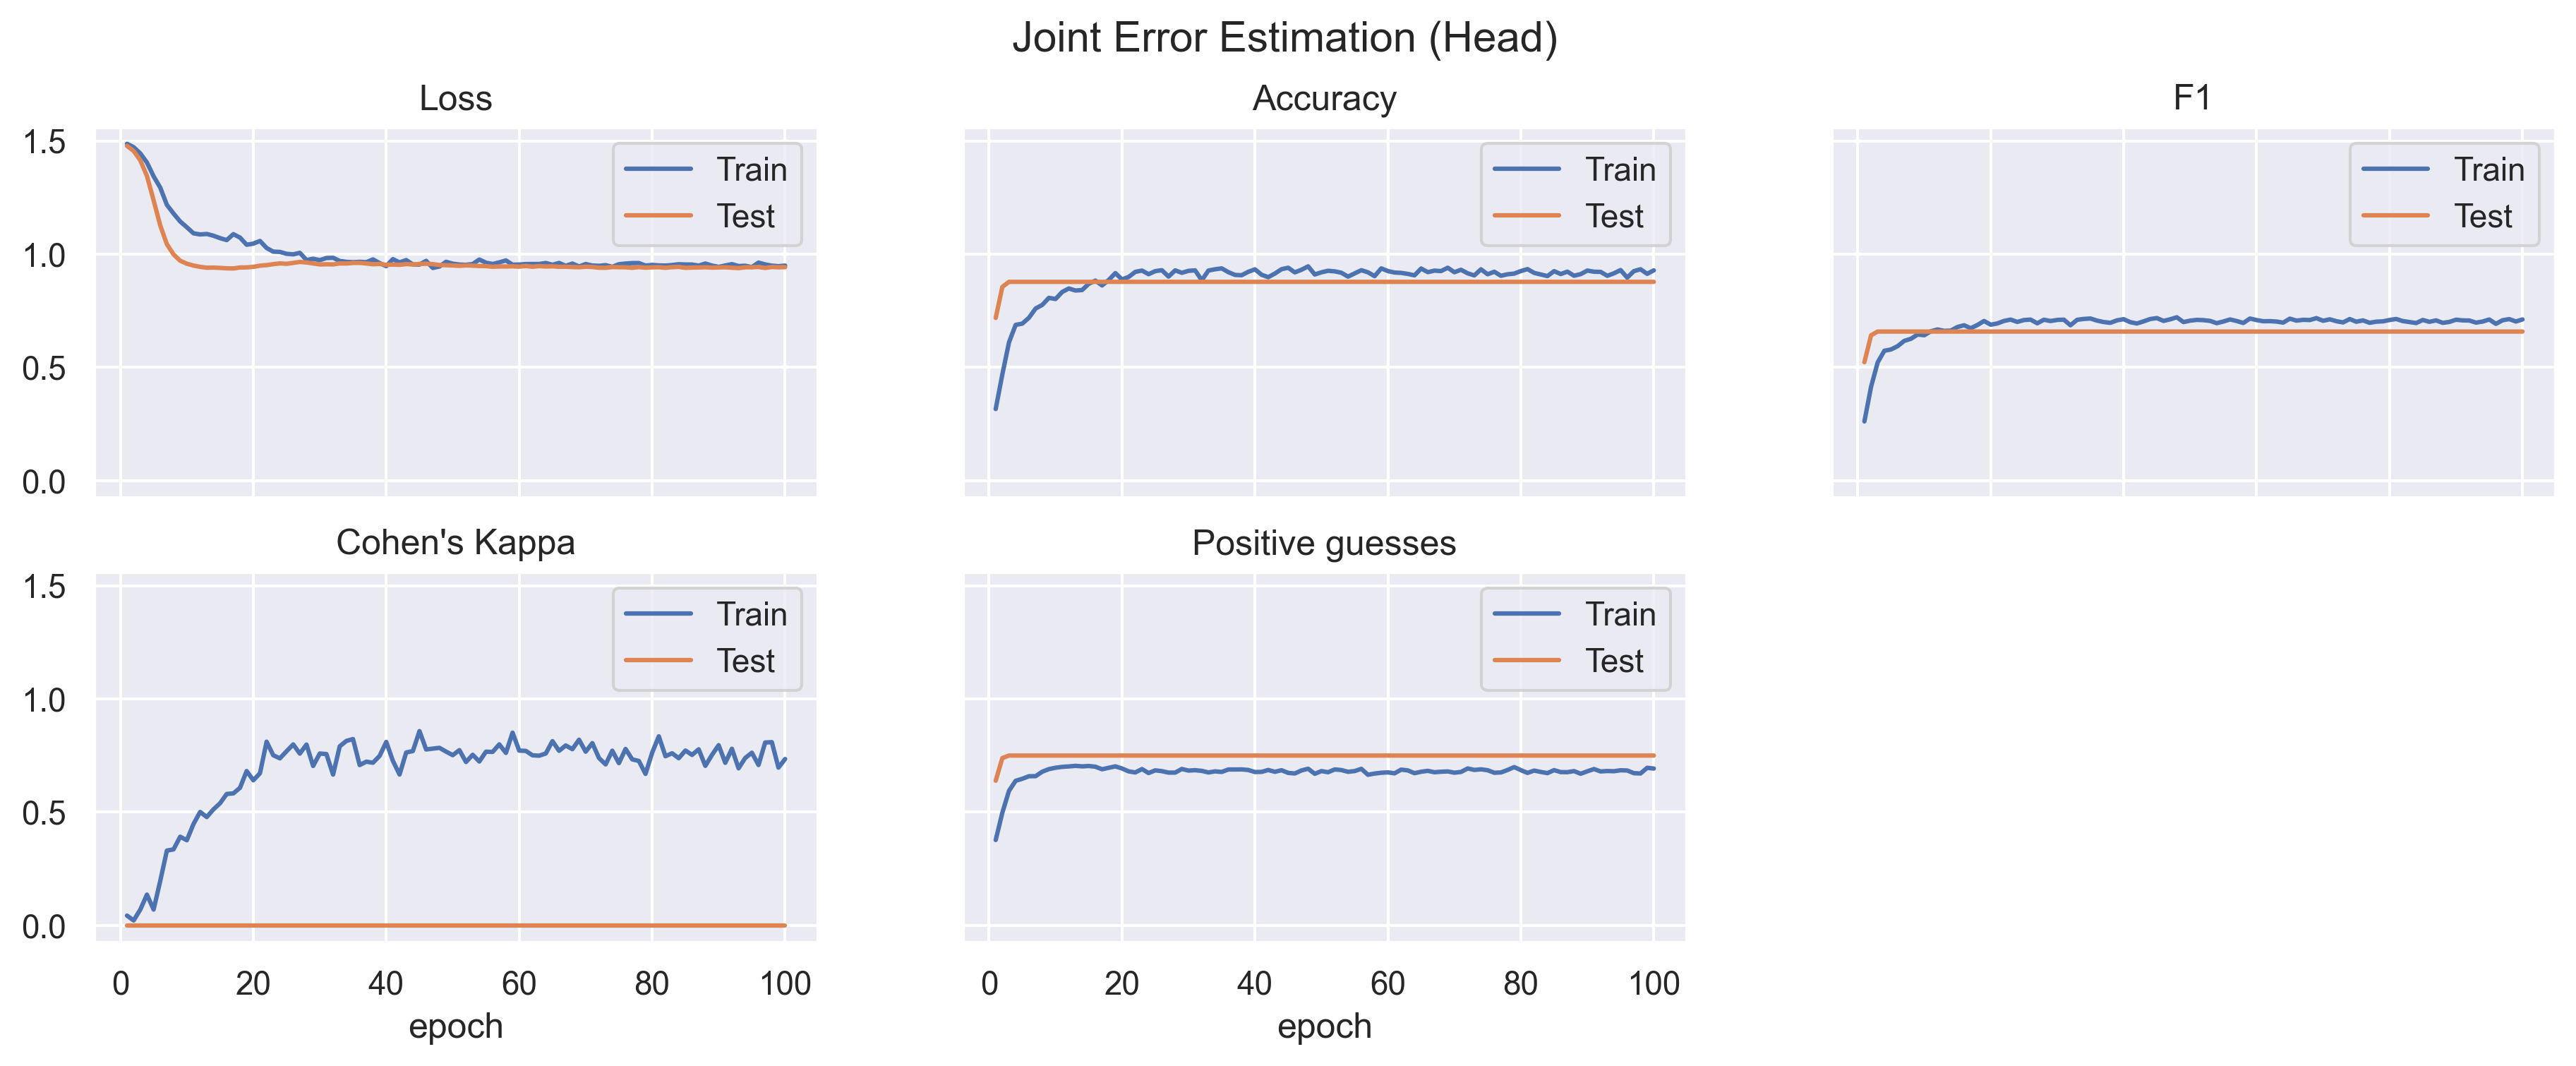
\includegraphics[width=\textwidth]{figures/Results/jt/JointErrorEstimation_Head.png}
      \caption{Head Error Estimation}
      \label{fig:head_jt_ee}
  \end{subfigure}
  \hfill
  \begin{subfigure}[b]{0.47\linewidth}
      \centering
      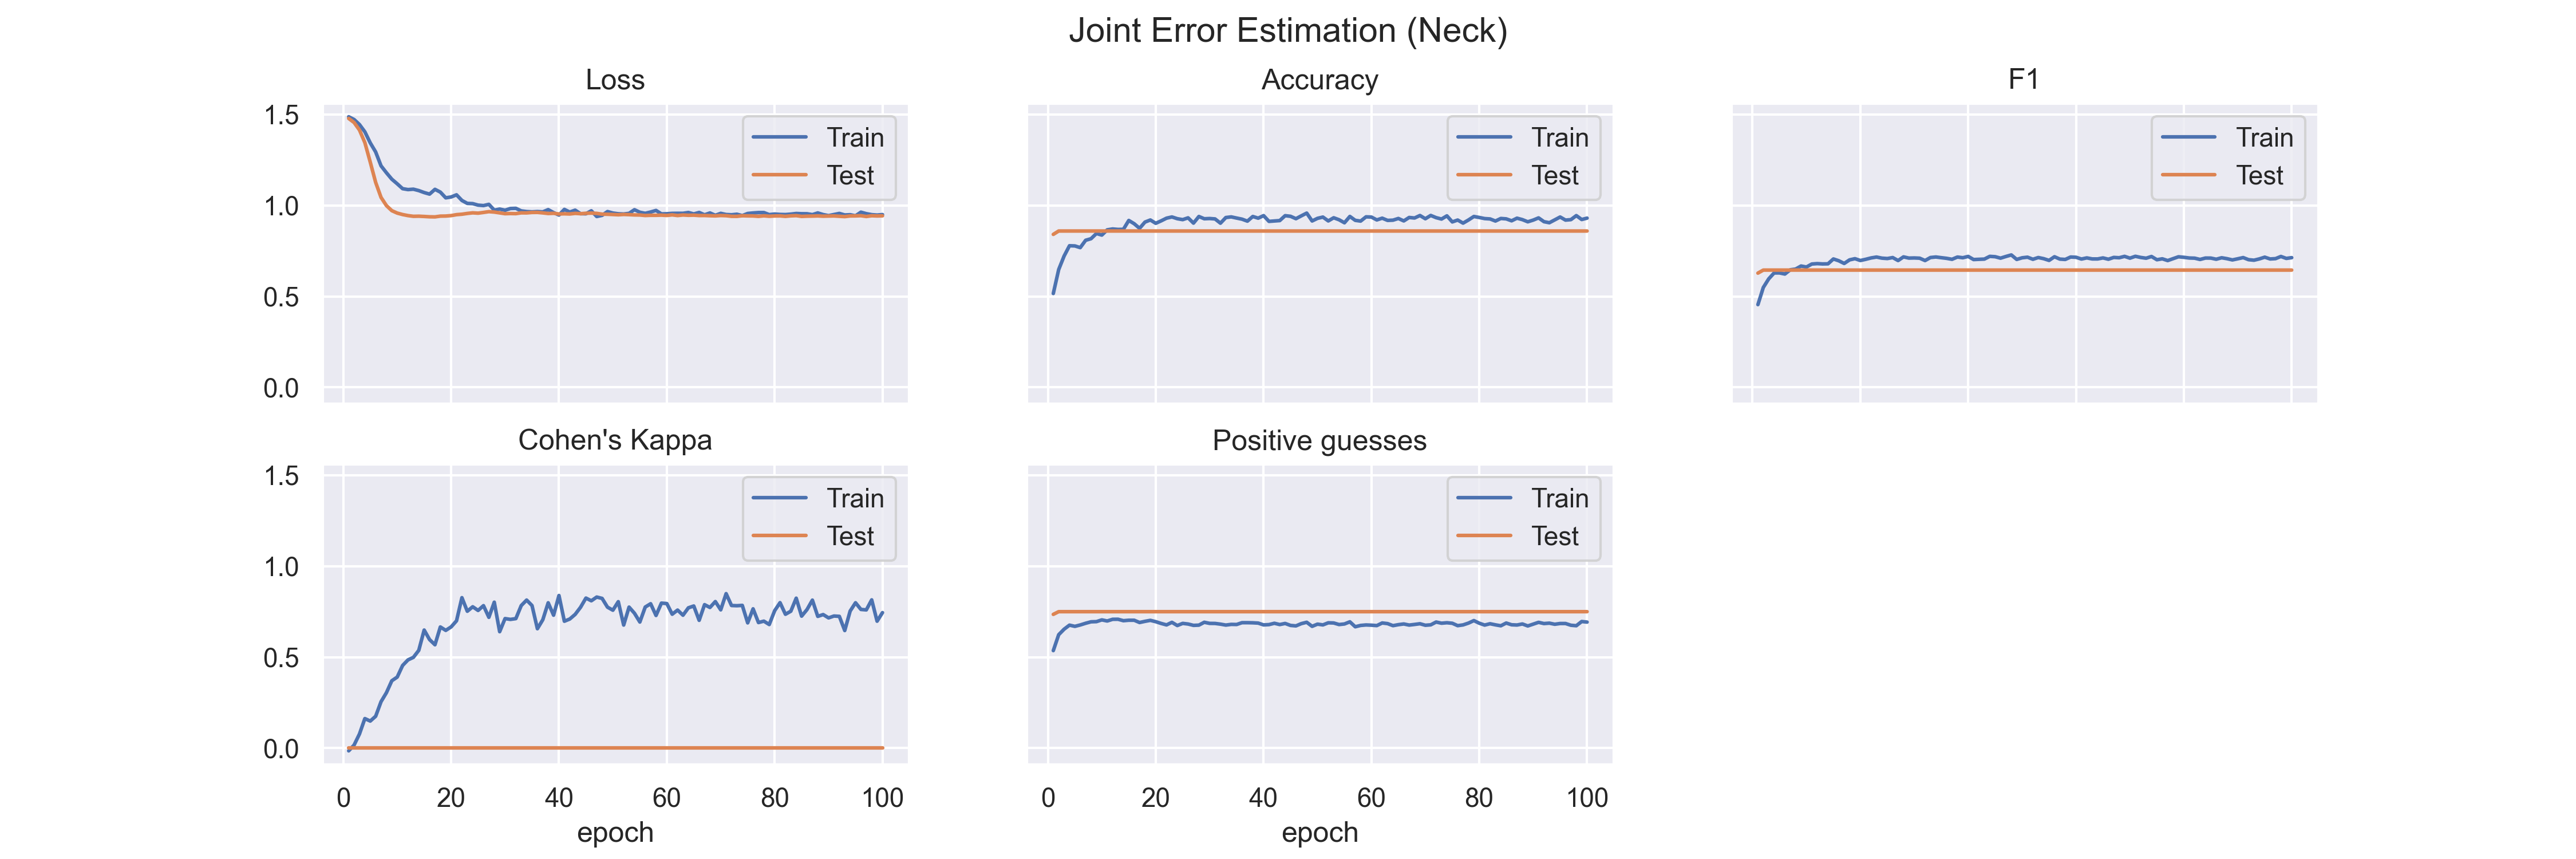
\includegraphics[width=\textwidth]{figures/Results/jt/JointErrorEstimation_Neck.png}
      \caption{Neck Error Estimation}
      \label{fig:neck_jt_ee}
  \end{subfigure}
  \hfill
  \begin{subfigure}[b]{0.47\linewidth}
      \centering
      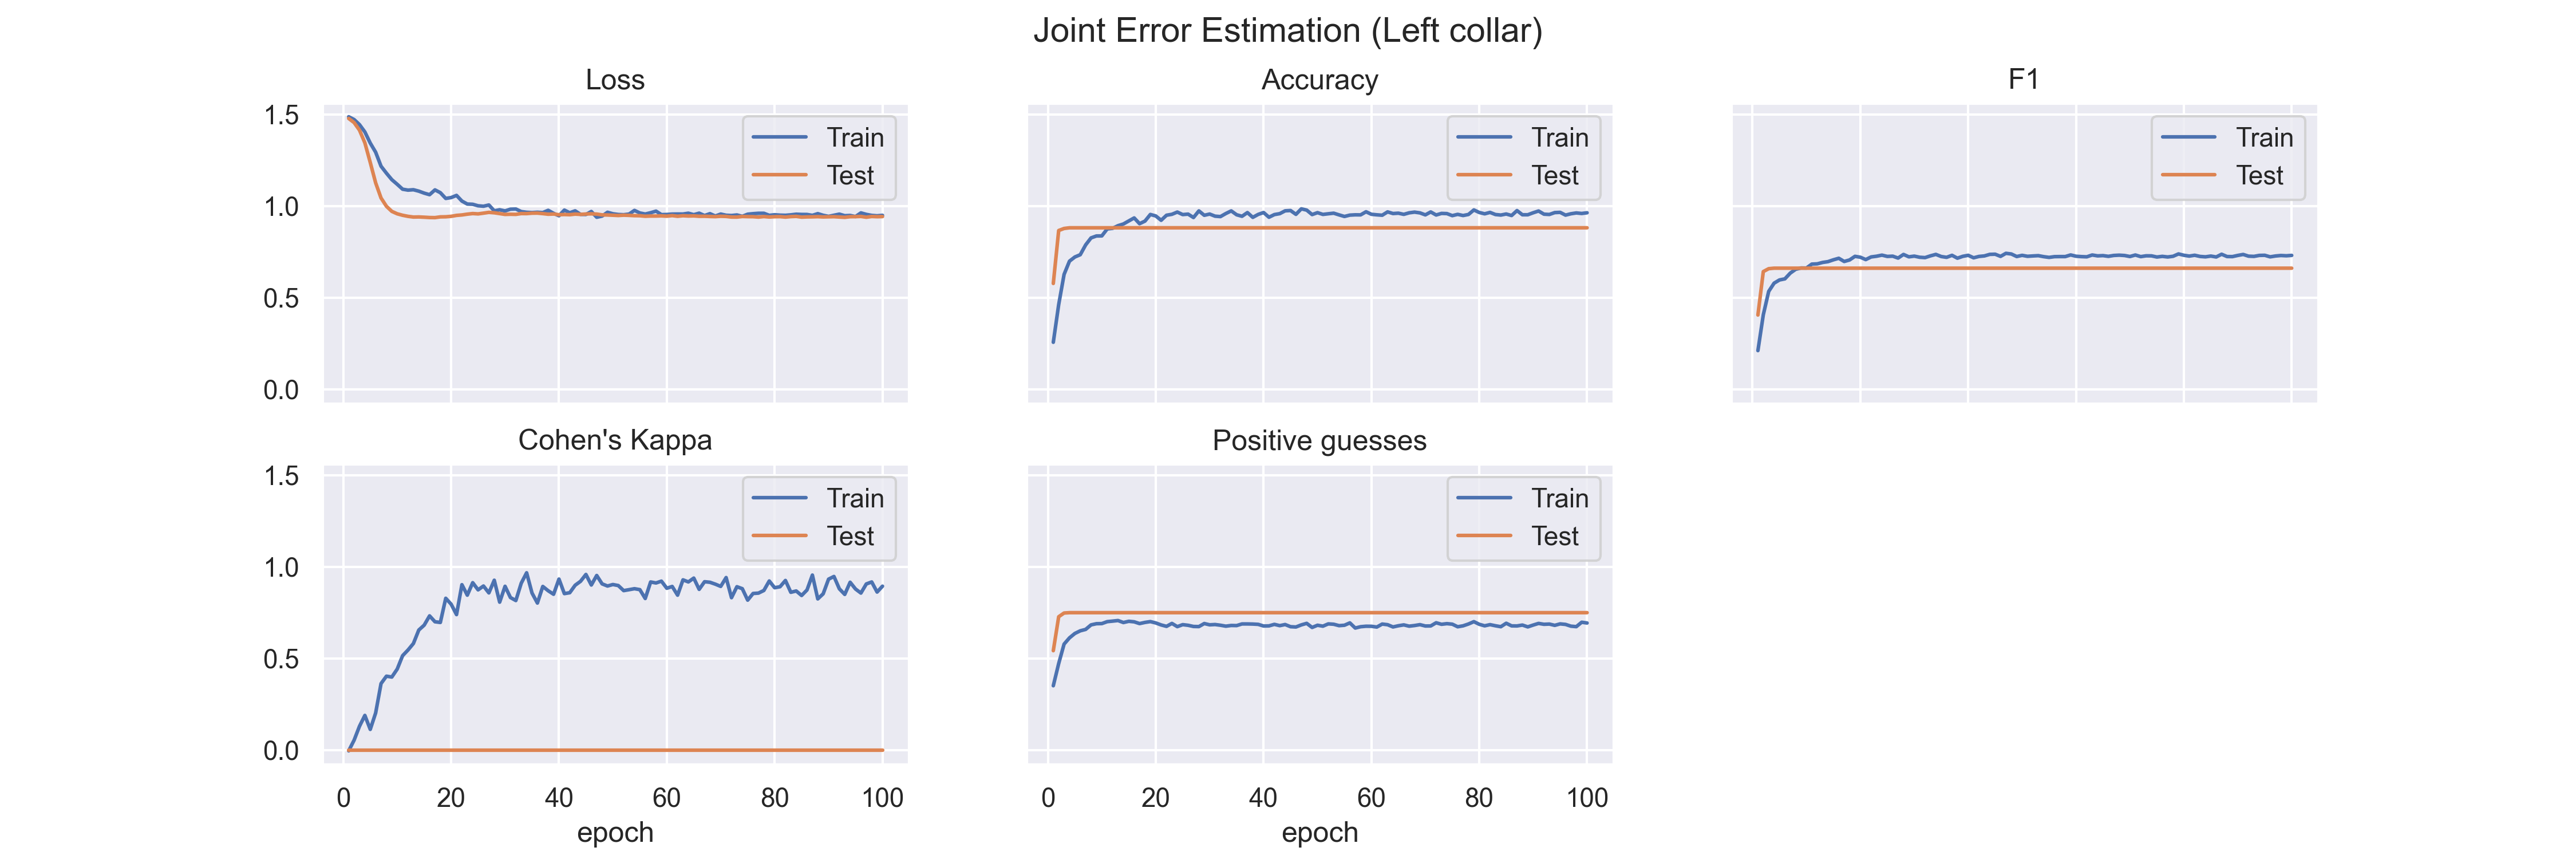
\includegraphics[width=\textwidth]{figures/Results/jt/JointErrorEstimation_Left collar.png}
      \caption{Left Collar Error Estimation}
      \label{fig:leco_jt_ee}
  \end{subfigure}
  \hfill
  \begin{subfigure}[b]{0.47\linewidth}
      \centering
      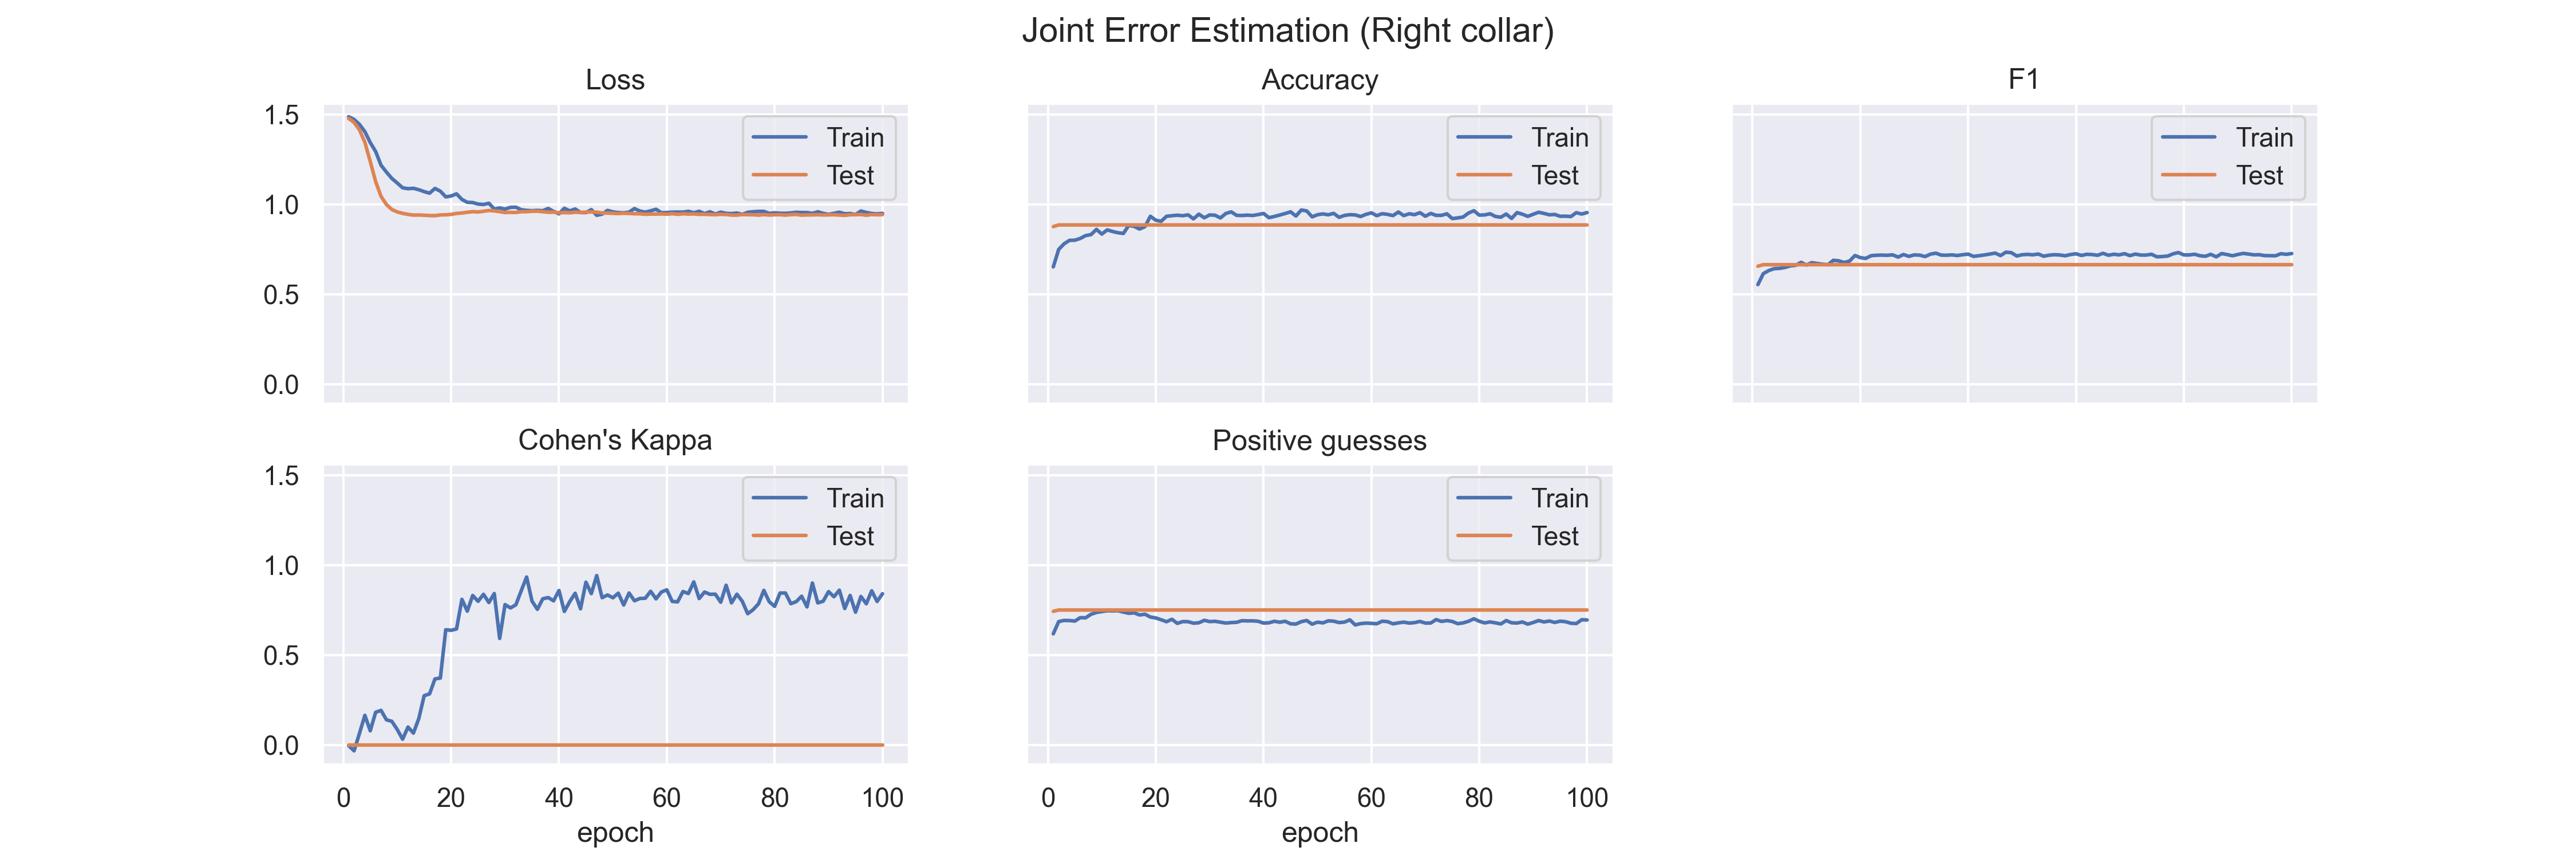
\includegraphics[width=\textwidth]{figures/Results/jt/JointErrorEstimation_Right collar.png}
      \caption{Right Collar Error Estimation}
      \label{fig:rico_jt_ee}
  \end{subfigure}
  \caption[Joint model training results]{The training results of the Joint error estimation model.}
  \label{fig:Joint_training_results}
\end{figure}


\begin{figure}
  \centering
  \begin{subfigure}[b]{0.47\linewidth}
      \centering
      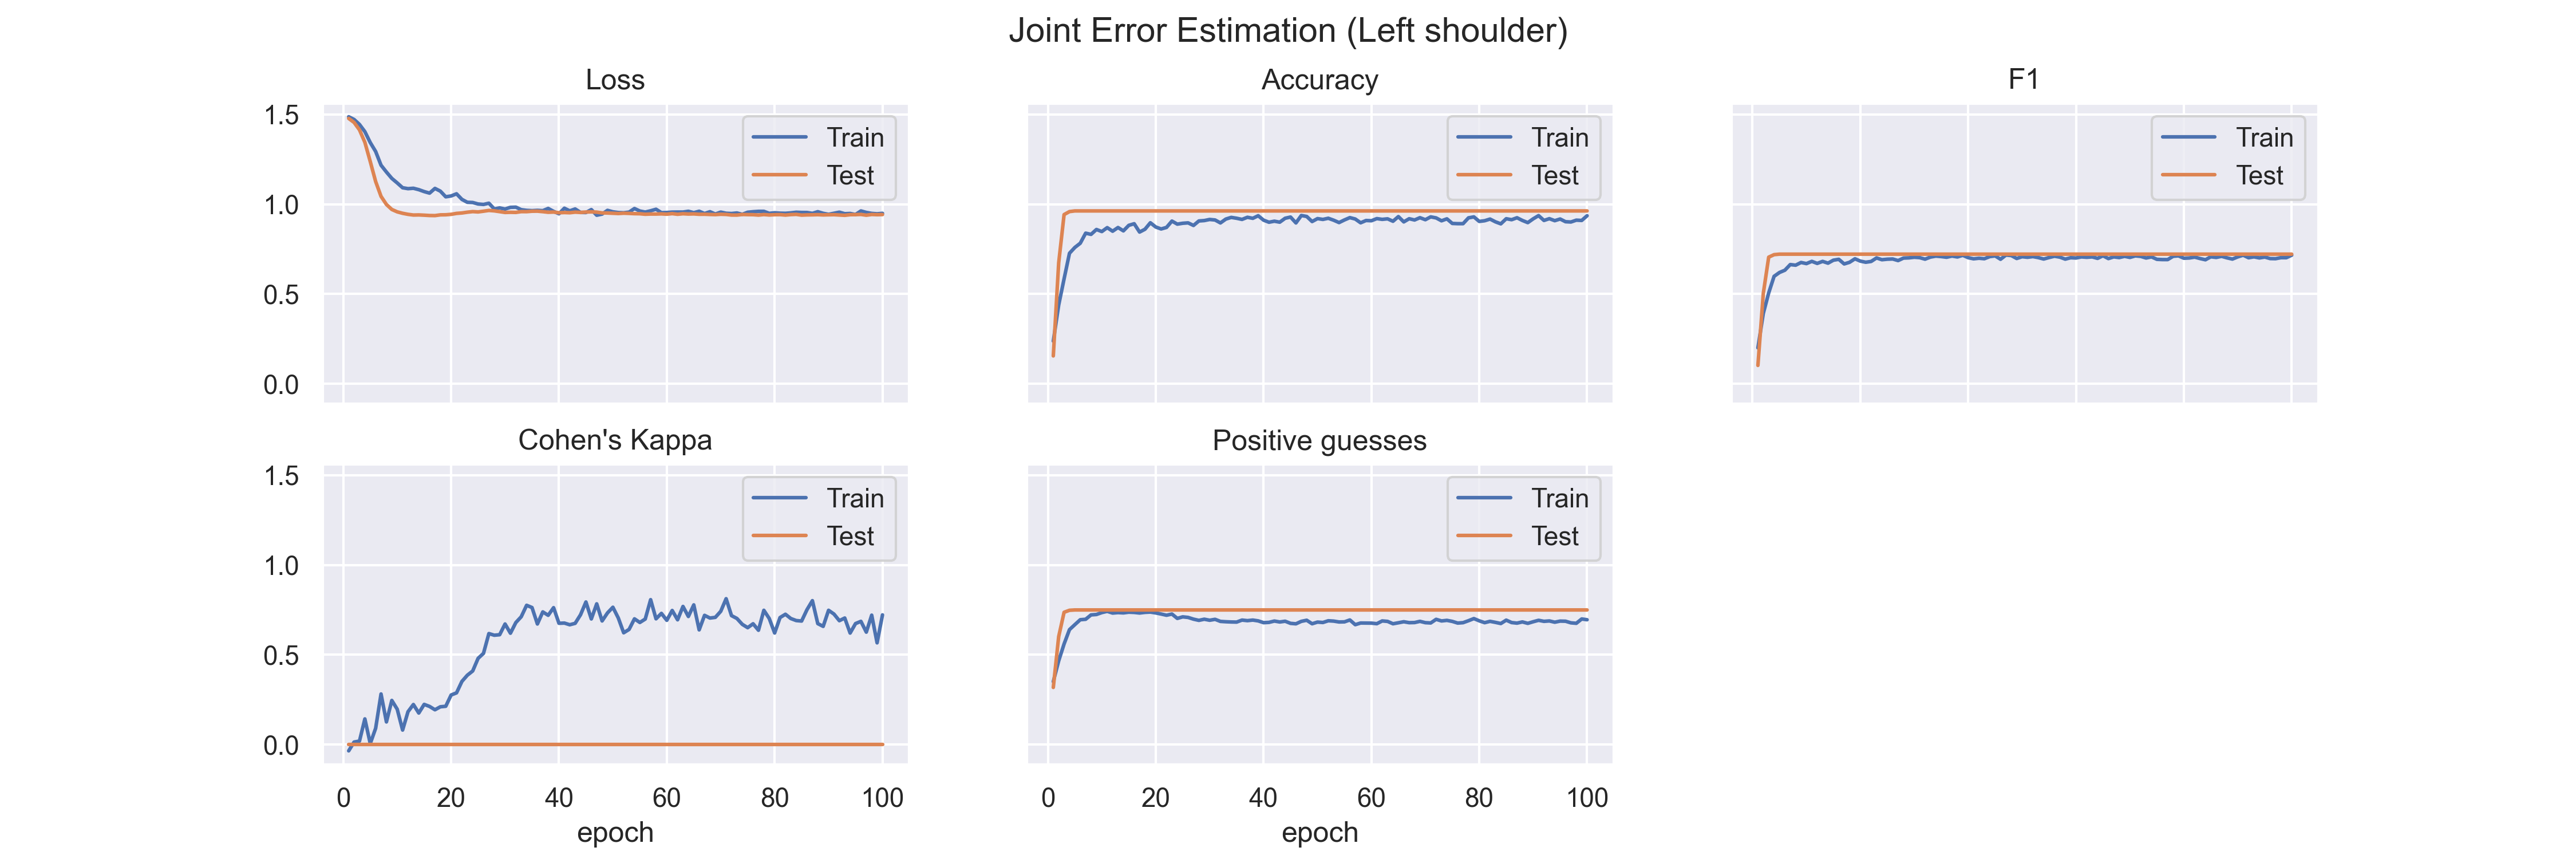
\includegraphics[width=\textwidth]{figures/Results/jt/JointErrorEstimation_Left shoulder.png}
      \caption{Left Shoulder Error Estimation}
      \label{fig:lesh_jt_ee}
  \end{subfigure}
  \hfill
  \begin{subfigure}[b]{0.47\linewidth}
      \centering
      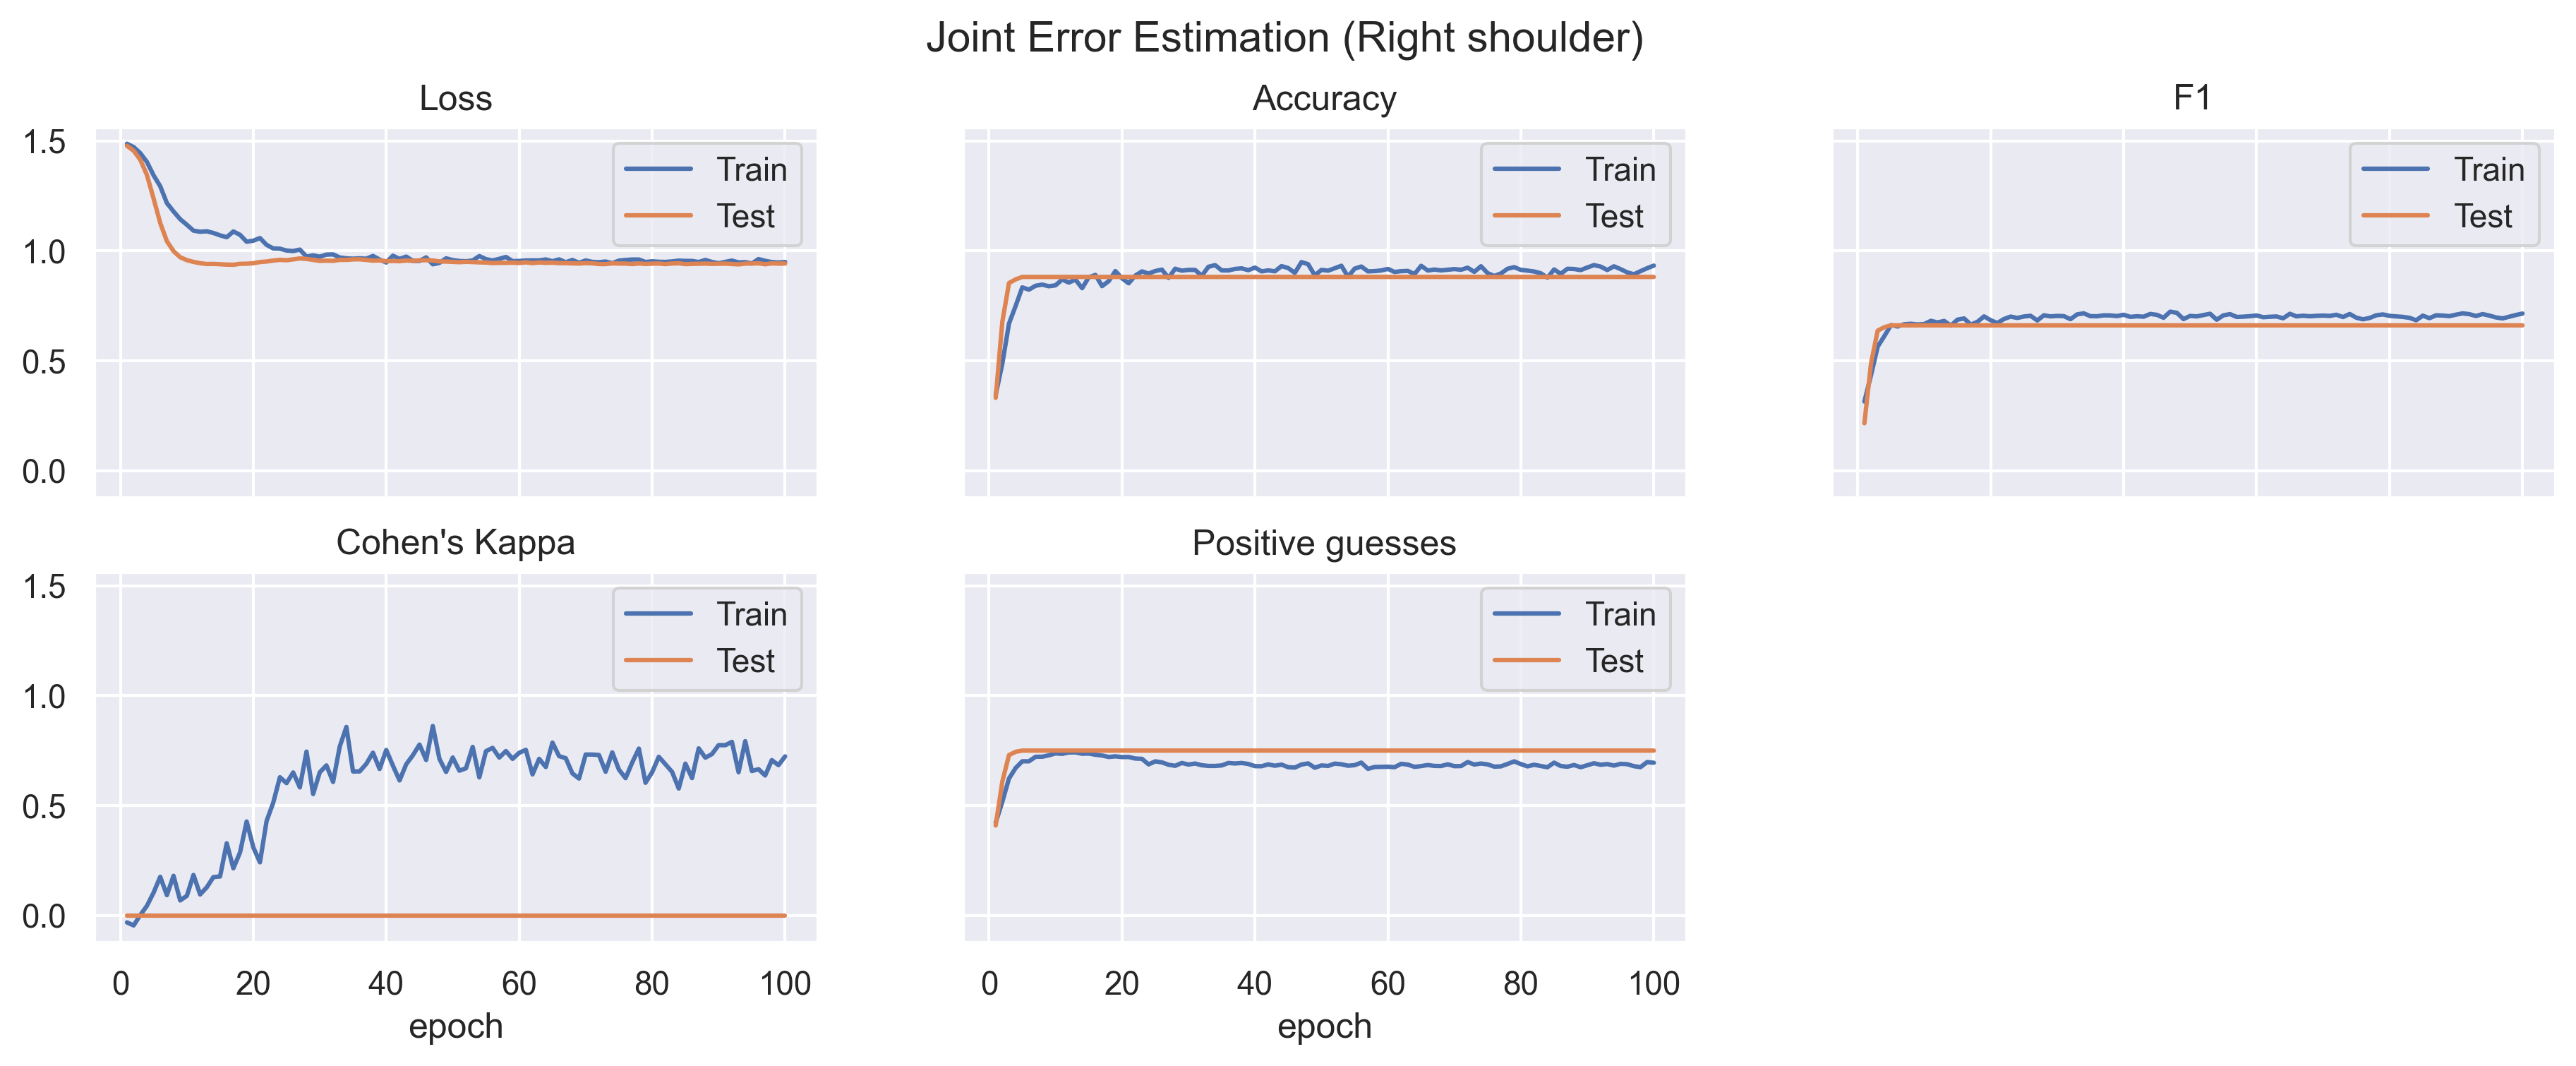
\includegraphics[width=\textwidth]{figures/Results/jt/JointErrorEstimation_Right shoulder.png}
      \caption{Right Shoulder Error Estimation}
      \label{fig:rish_jt_ee}
  \end{subfigure}
  \hfill
  \begin{subfigure}[b]{0.47\linewidth}
      \centering
      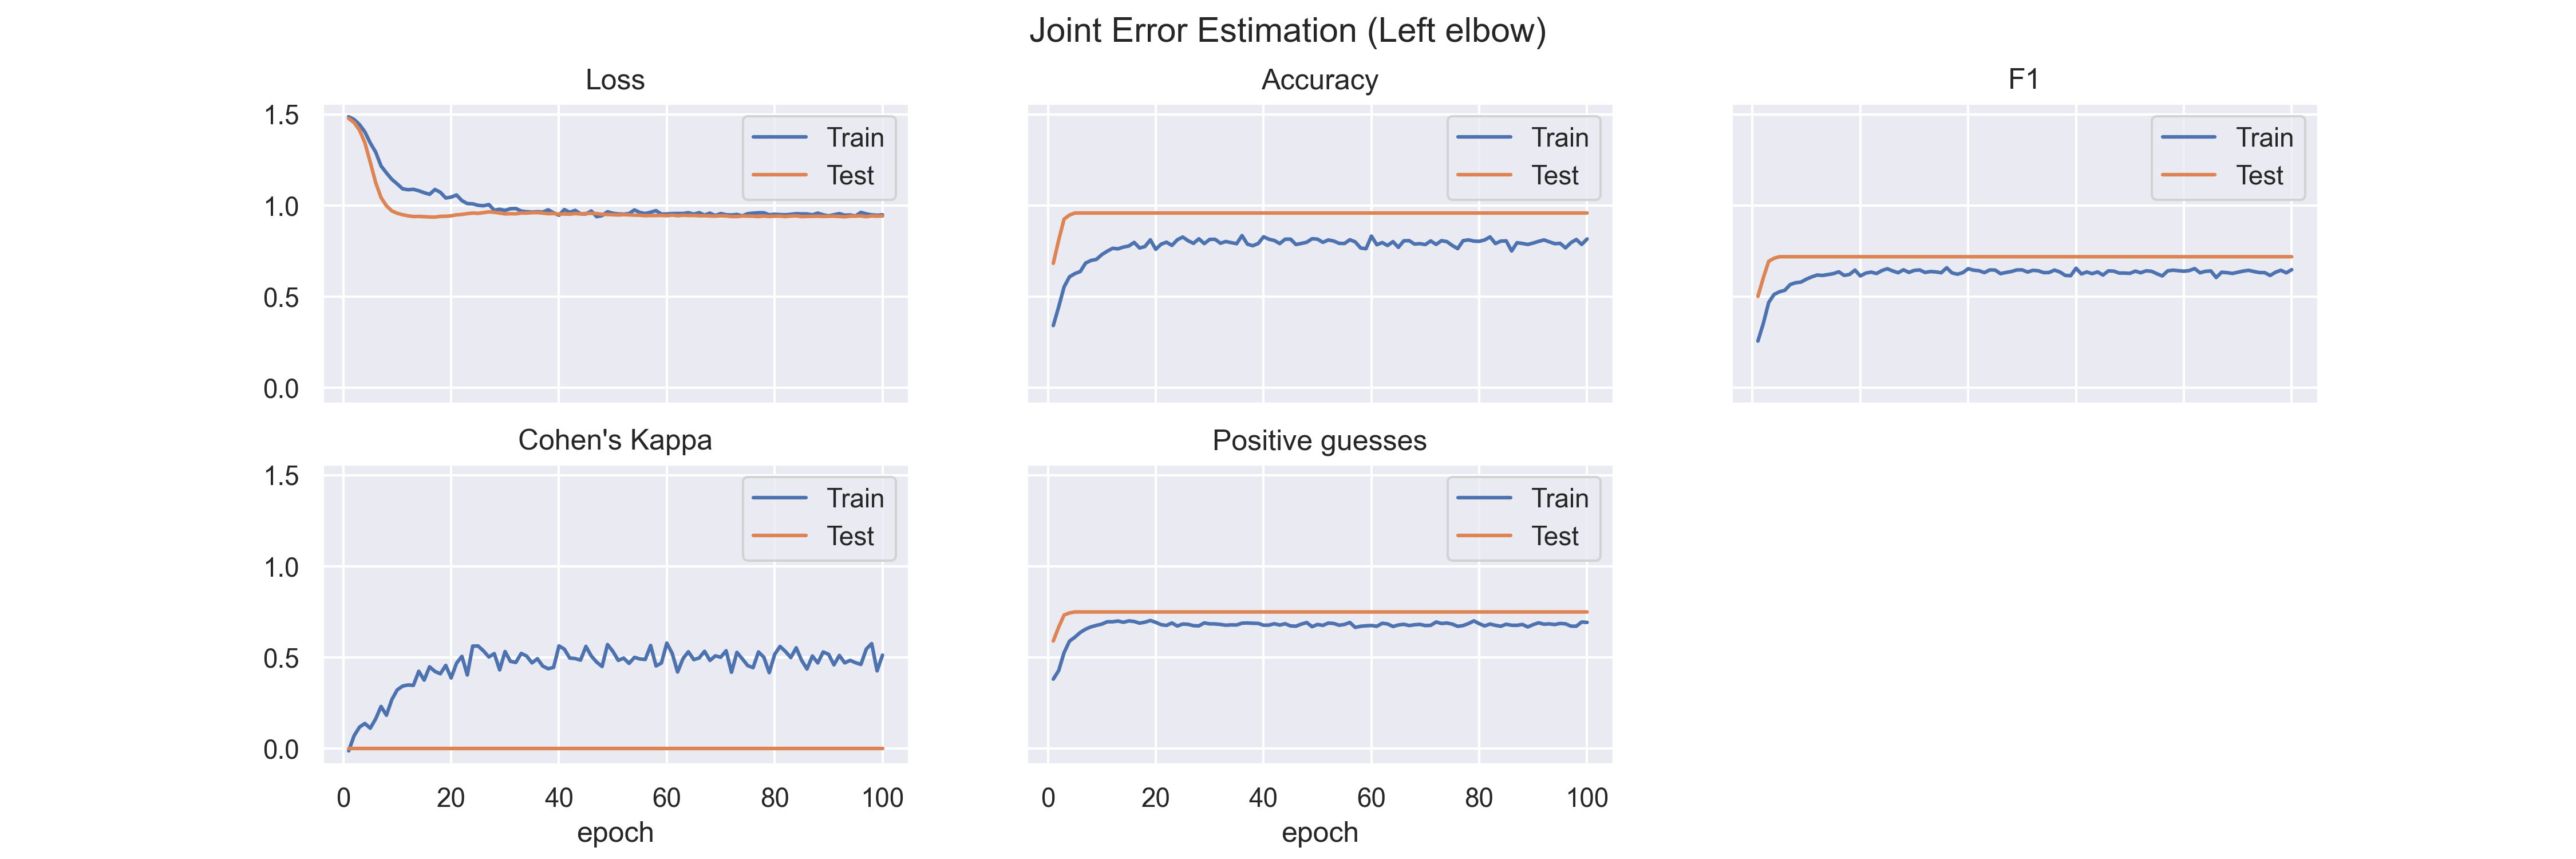
\includegraphics[width=\textwidth]{figures/Results/jt/JointErrorEstimation_Left elbow.png}
      \caption{Left Elbow Error Estimation}
      \label{fig:leel_jt_ee}
  \end{subfigure}
  \hfill
  \begin{subfigure}[b]{0.47\linewidth}
      \centering
      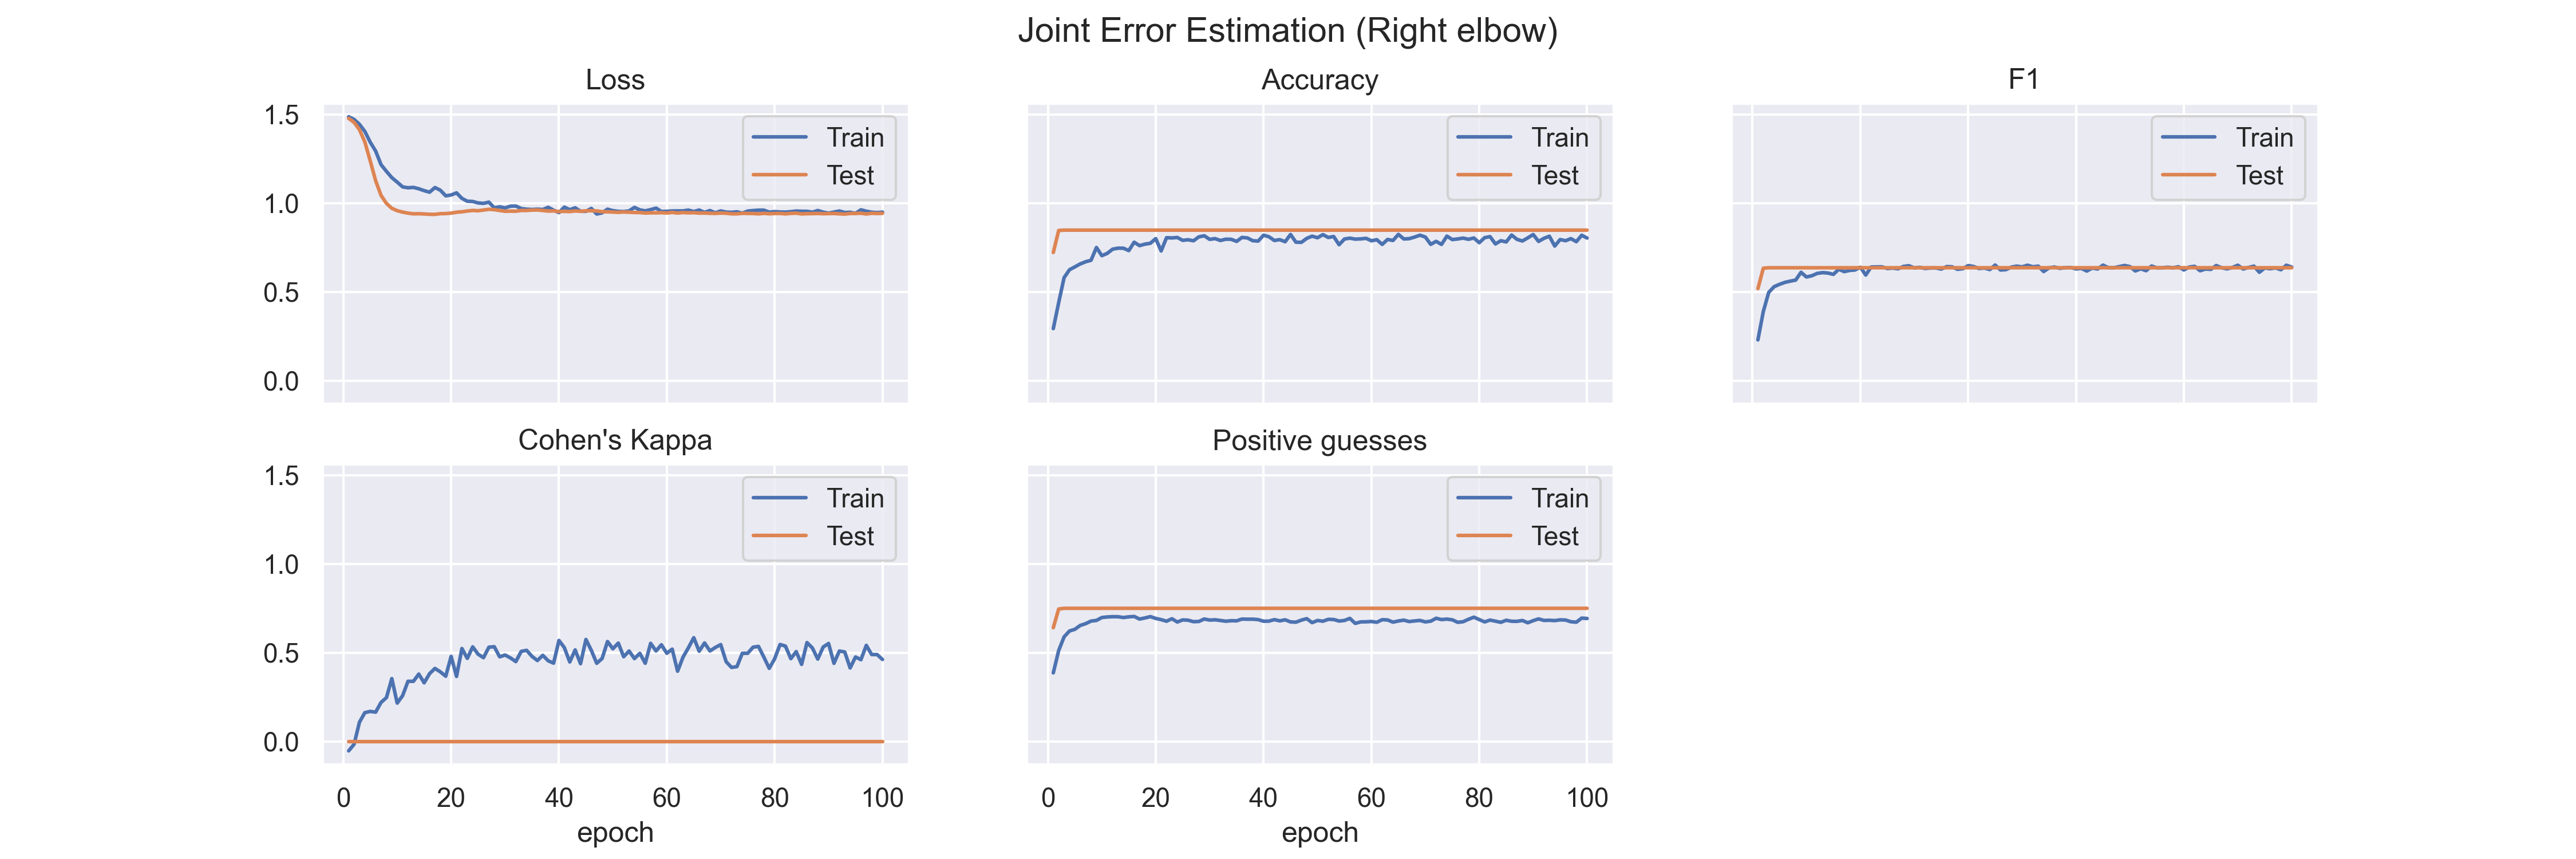
\includegraphics[width=\textwidth]{figures/Results/jt/JointErrorEstimation_Right elbow.png}
      \caption{Right Elbow Error Estimation}
      \label{fig:reel_jt_ee}
  \end{subfigure}
  \caption[Joint model training results]{The training results of the Joint error estimation model. (cont. 1)}
  \label{fig:Joint_training_results_1}
\end{figure}


\begin{figure}
  \centering
  \begin{subfigure}[b]{0.47\linewidth}
      \centering
      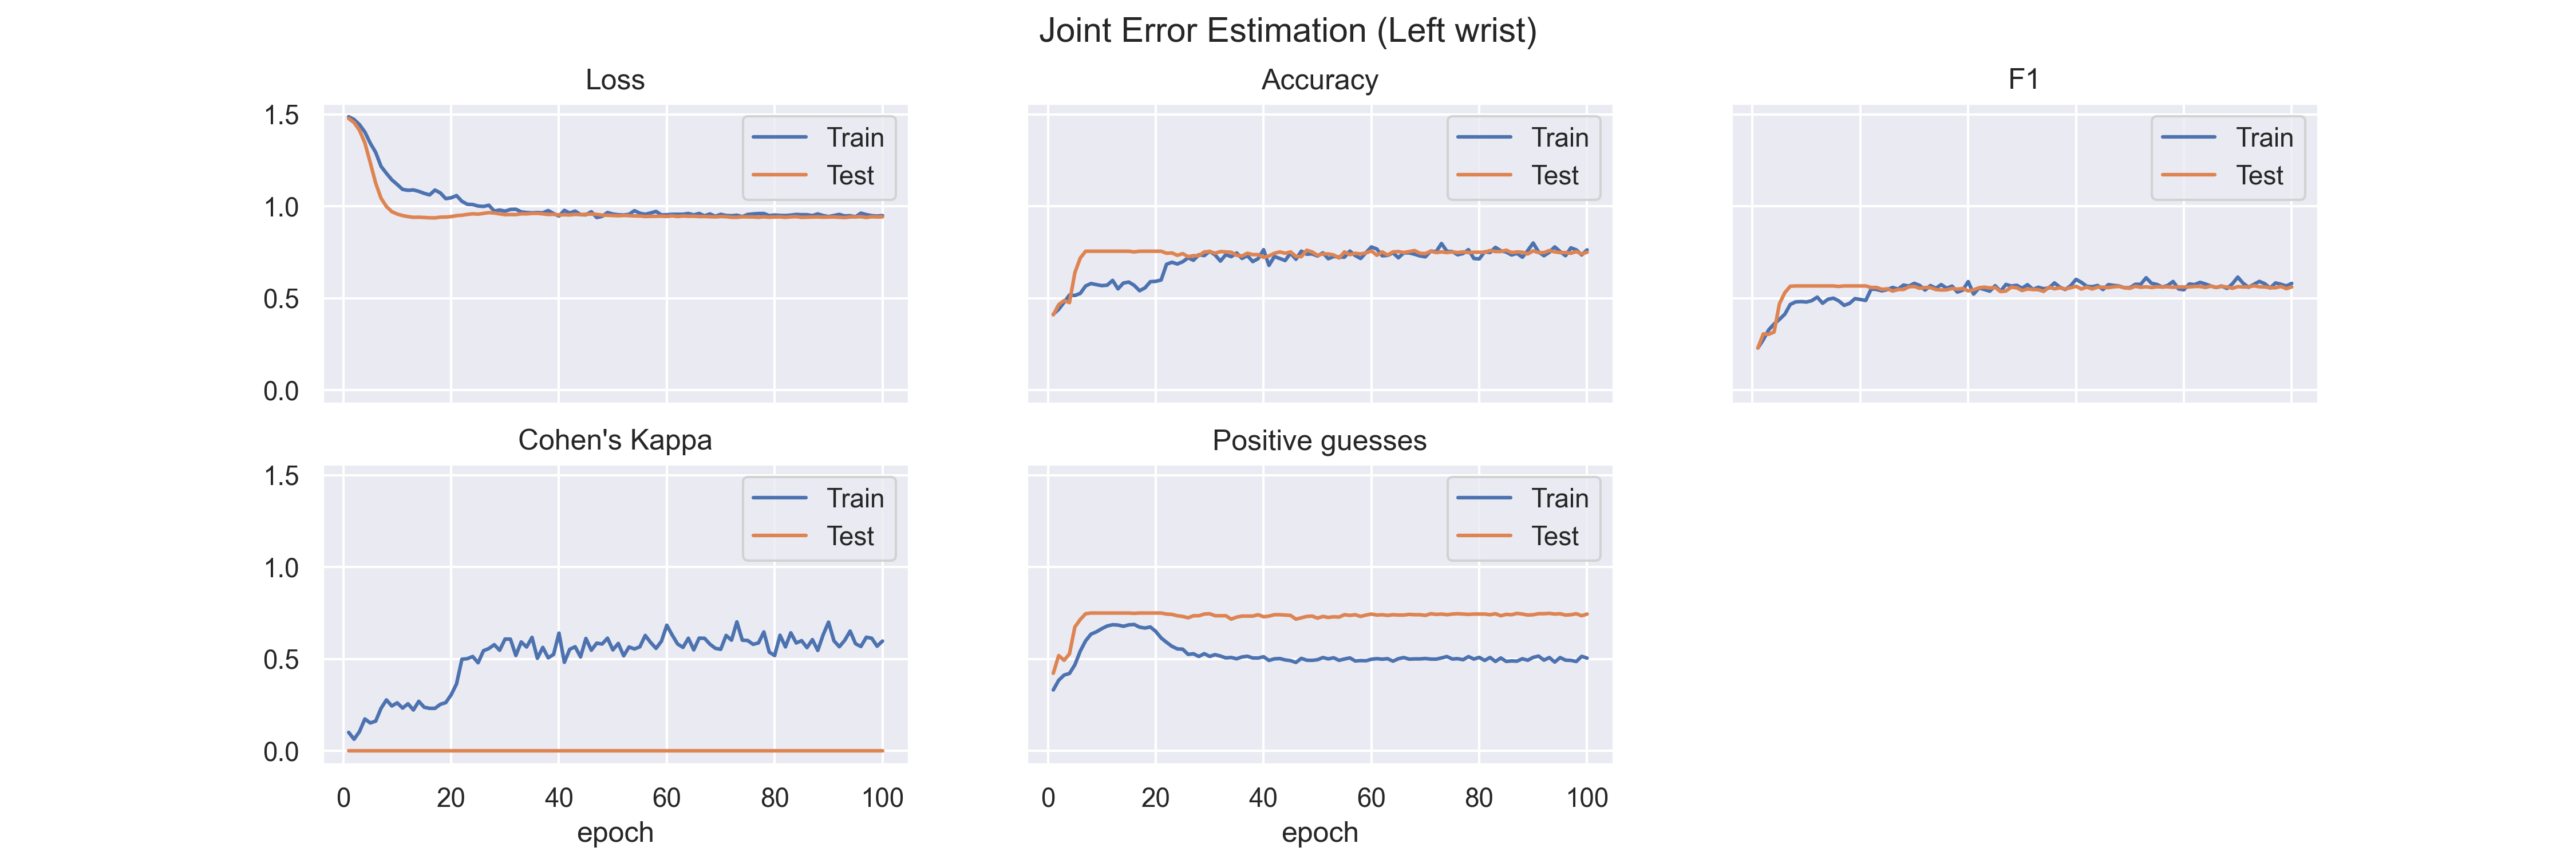
\includegraphics[width=\textwidth]{figures/Results/jt/JointErrorEstimation_Left wrist.png}
      \caption{Left Wrist Error Estimation}
      \label{fig:lewr_jt_ee}
  \end{subfigure}
  \hfill
  \begin{subfigure}[b]{0.47\linewidth}
      \centering
      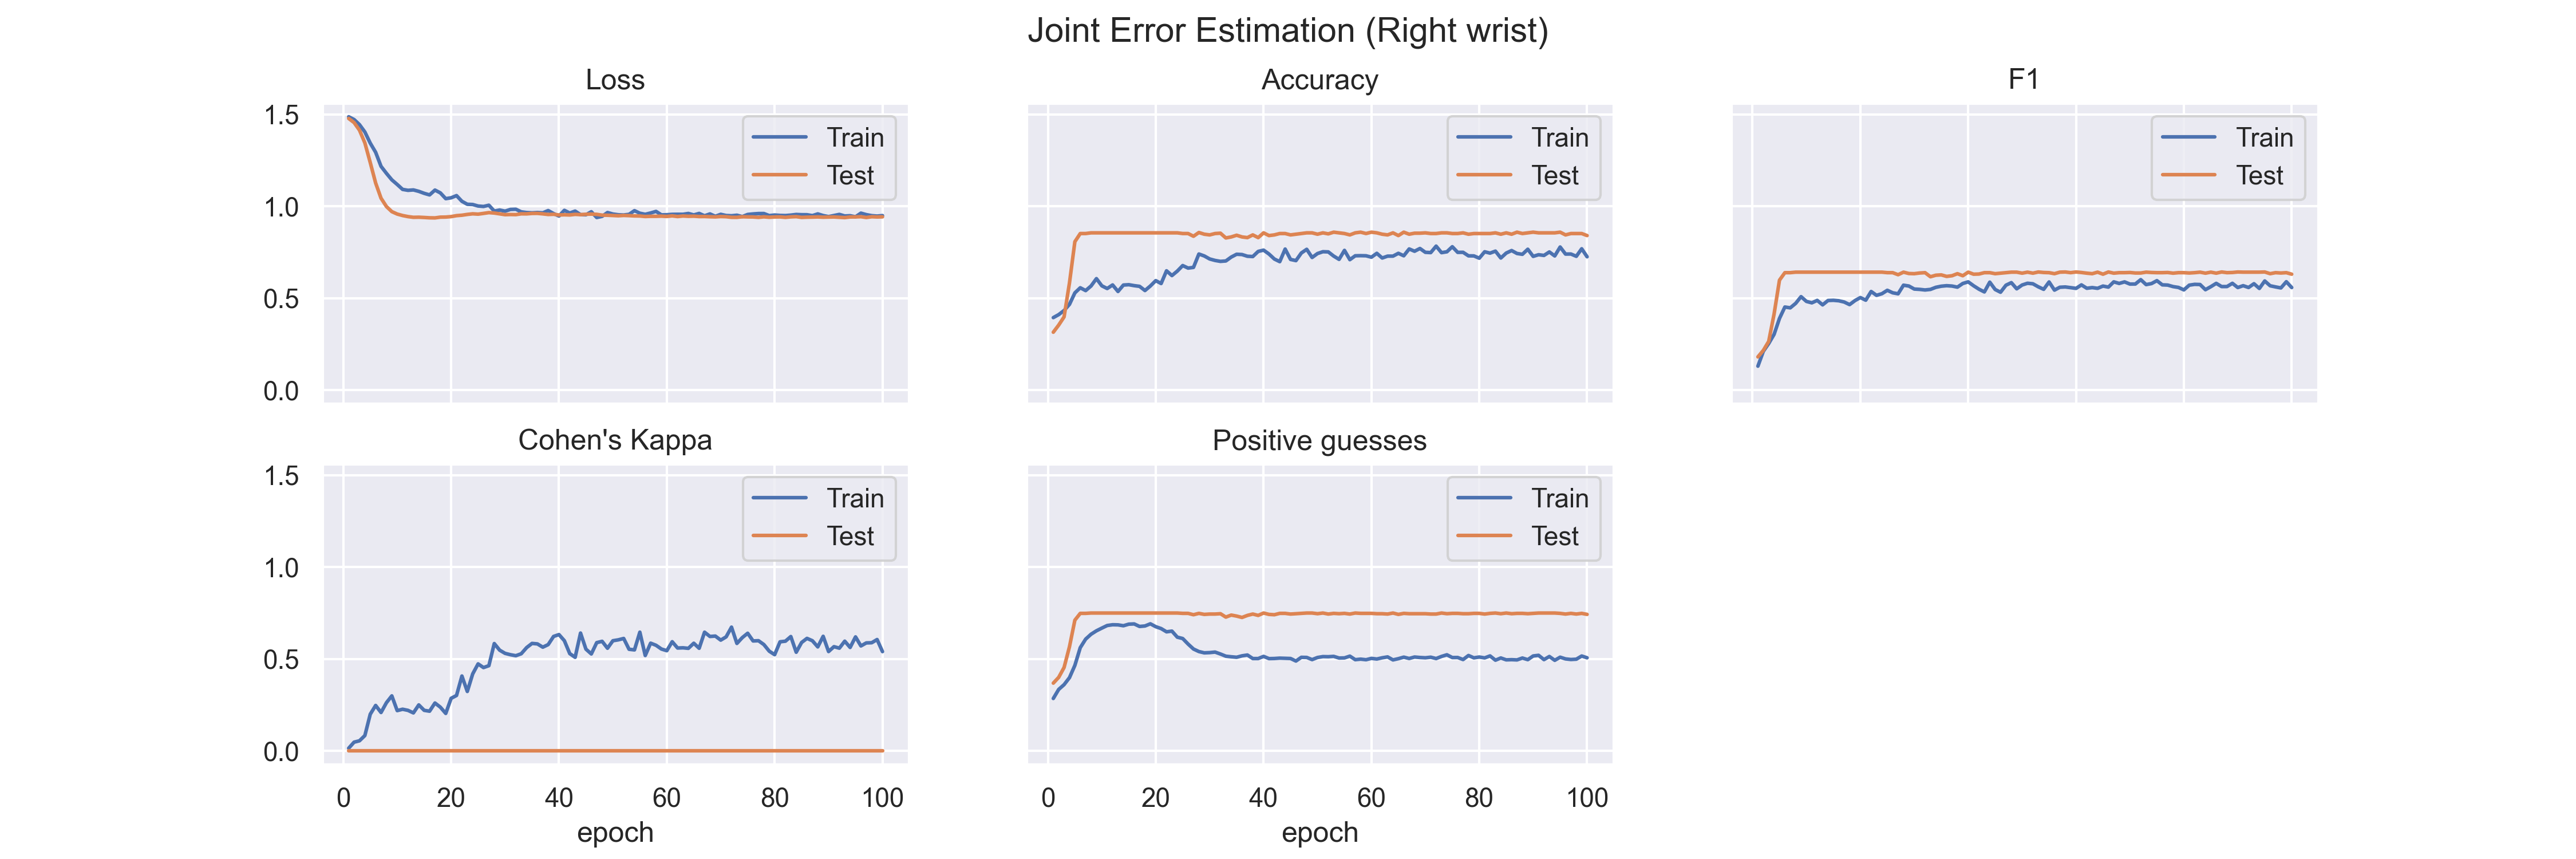
\includegraphics[width=\textwidth]{figures/Results/jt/JointErrorEstimation_Right wrist.png}
      \caption{Right Wrist Error Estimation}
      \label{fig:riwr_jt_ee}
  \end{subfigure}
  \hfill
  \begin{subfigure}[b]{0.47\linewidth}
      \centering
      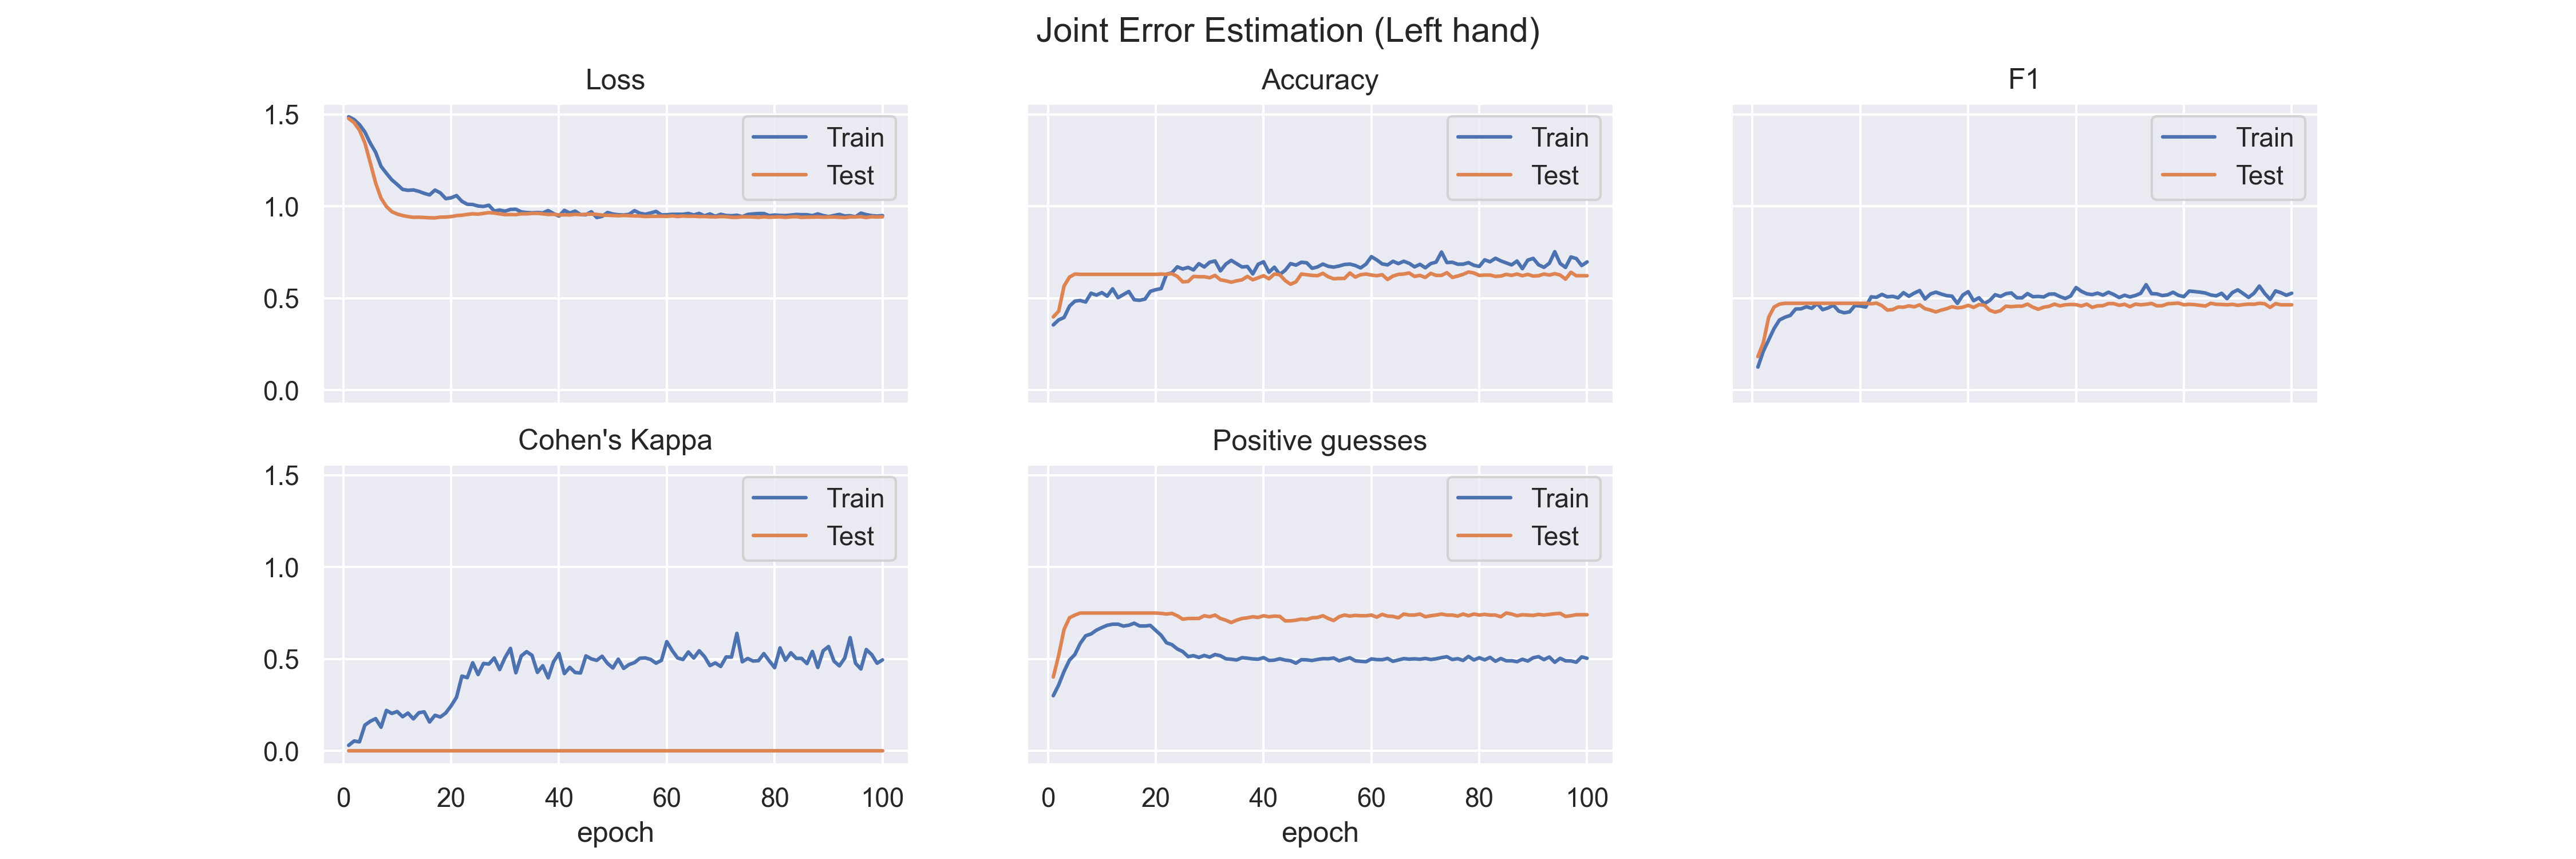
\includegraphics[width=\textwidth]{figures/Results/jt/JointErrorEstimation_Left hand.png}
      \caption{Left Hand Error Estimation}
      \label{fig:leha_jt_ee}
  \end{subfigure}
  \hfill
  \begin{subfigure}[b]{0.47\linewidth}
      \centering
      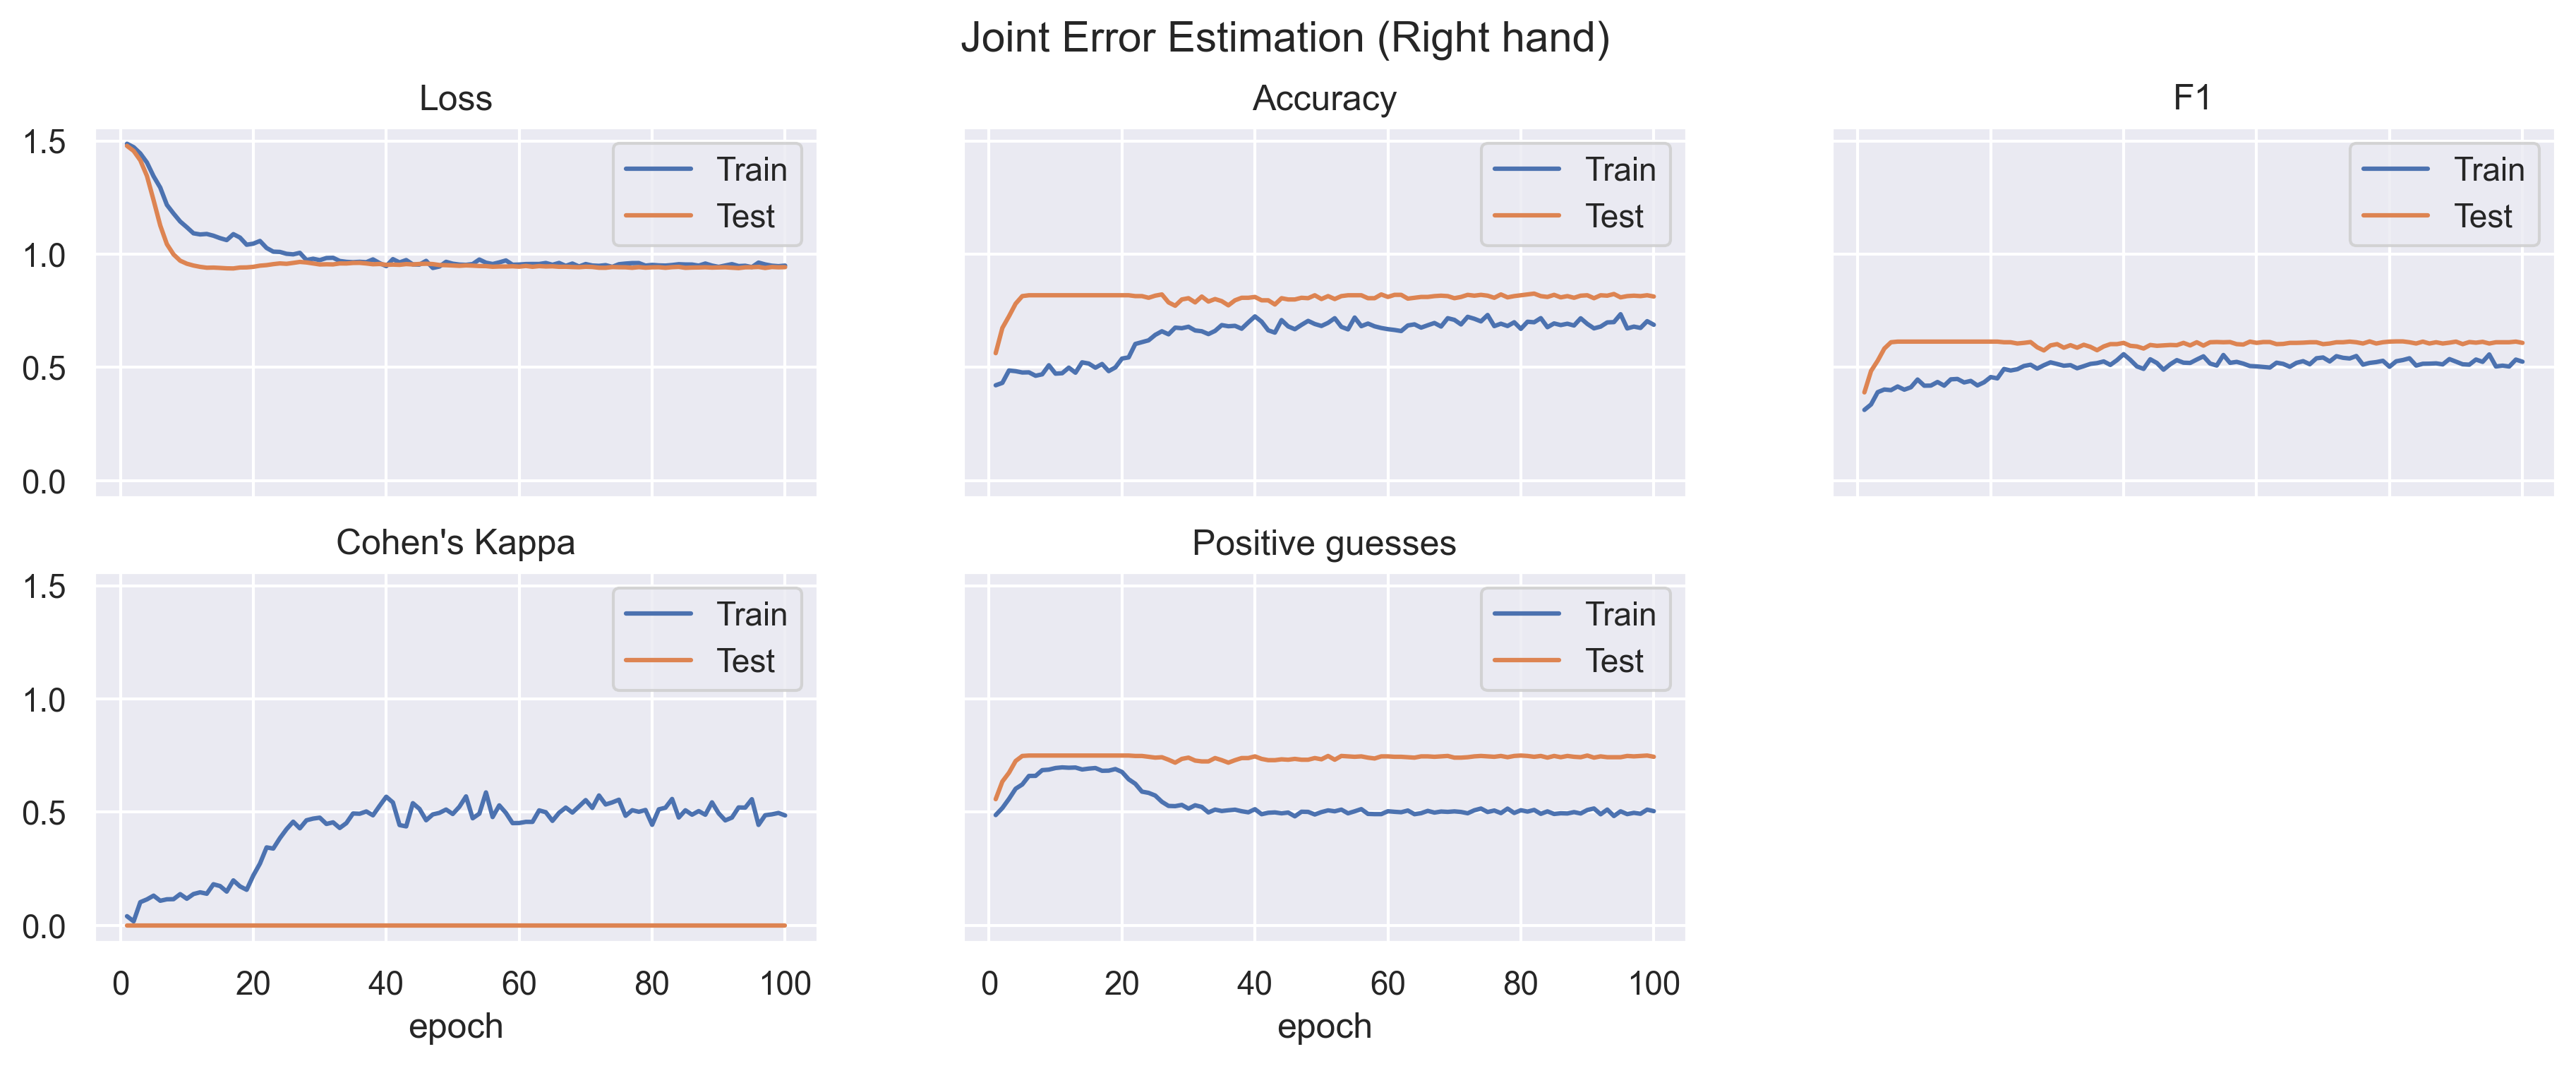
\includegraphics[width=\textwidth]{figures/Results/jt/JointErrorEstimation_Right hand.png}
      \caption{Left Arm Error Estimation}
      \label{fig:riha_jt_ee}
  \end{subfigure}
  \caption[Joint model training results]{The training results of the Joint error estimation model. (cont. 2)}
\end{figure}

\begin{figure}
  \centering
  \begin{subfigure}[b]{0.47\linewidth}
      \centering
      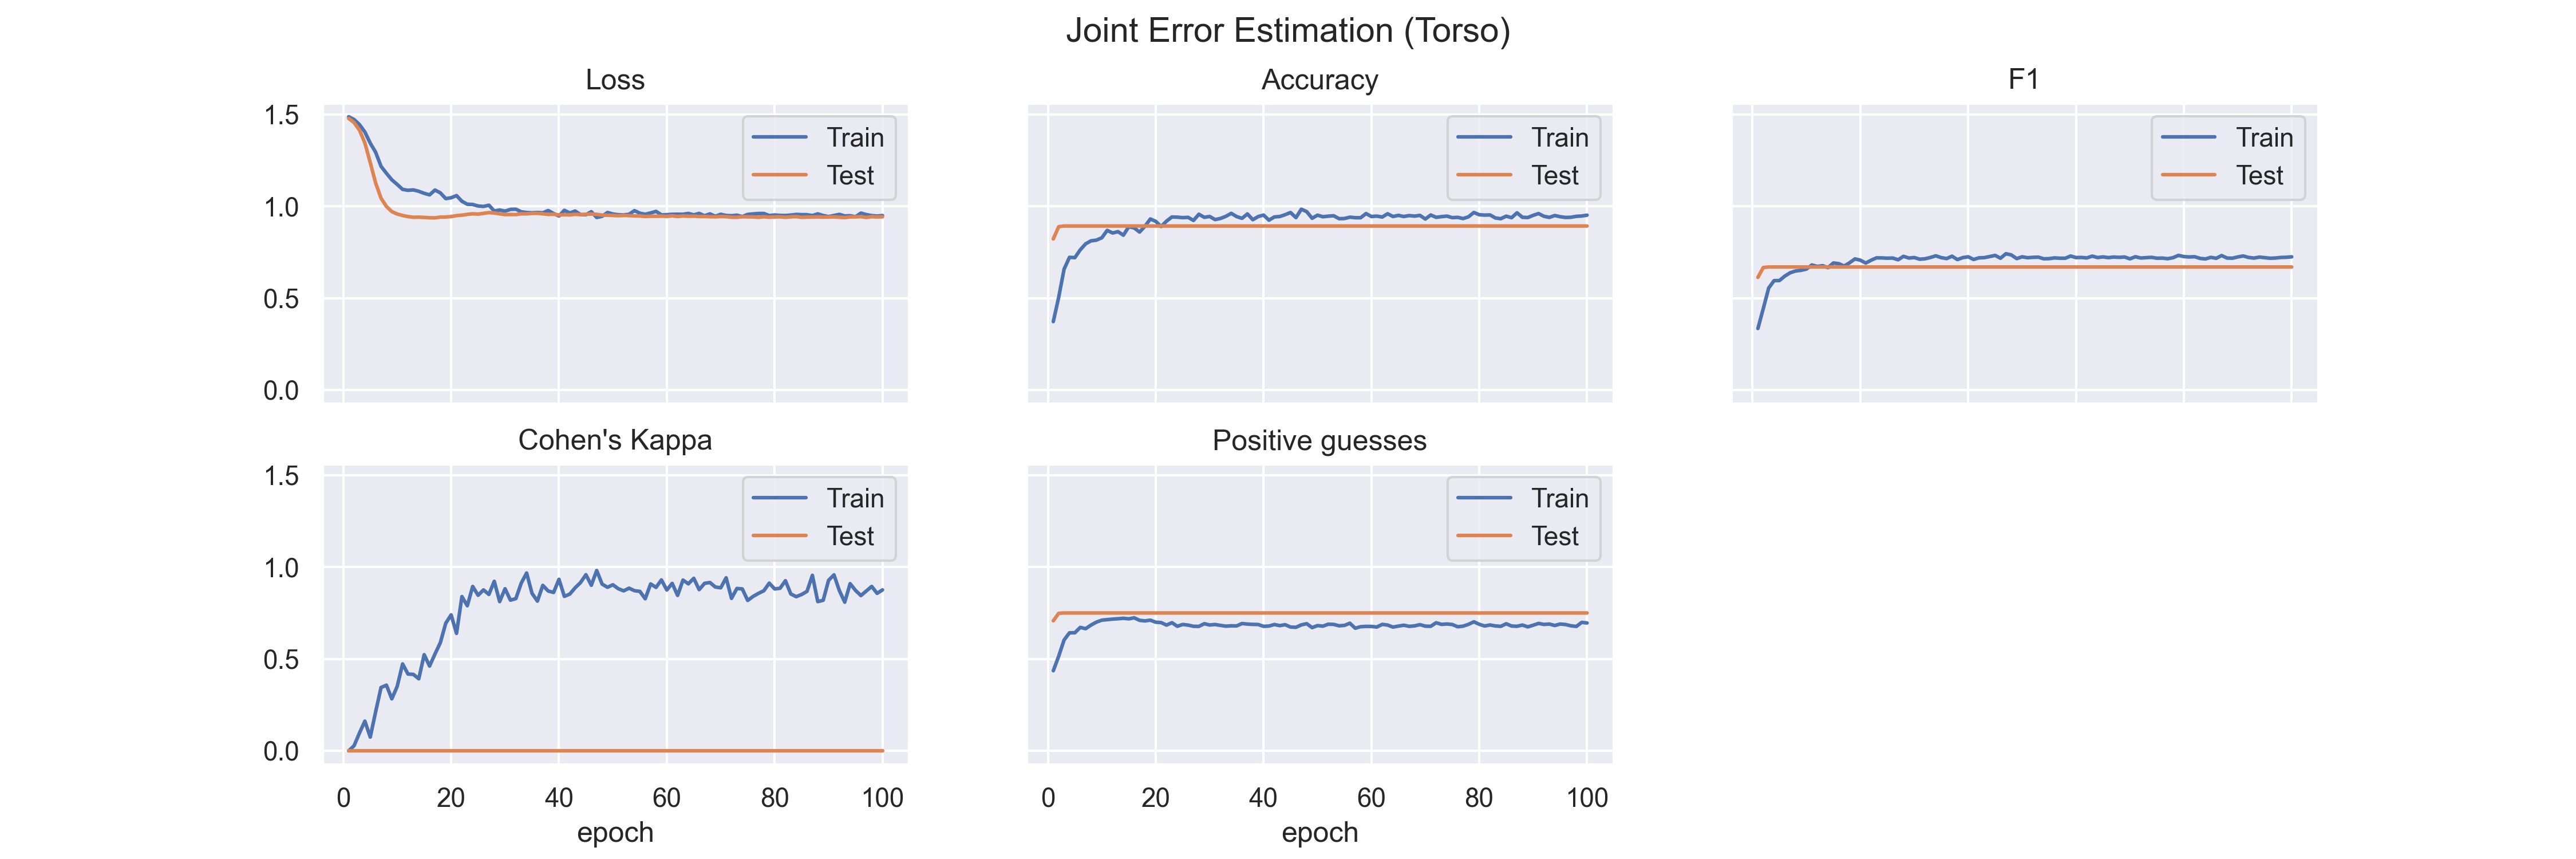
\includegraphics[width=\textwidth]{figures/Results/jt/JointErrorEstimation_Torso.png}
      \caption{Torso Error Estimation}
      \label{fig:torso_jt_ee}
  \end{subfigure}
  \hfill
  \begin{subfigure}[b]{0.47\linewidth}
    \centering
    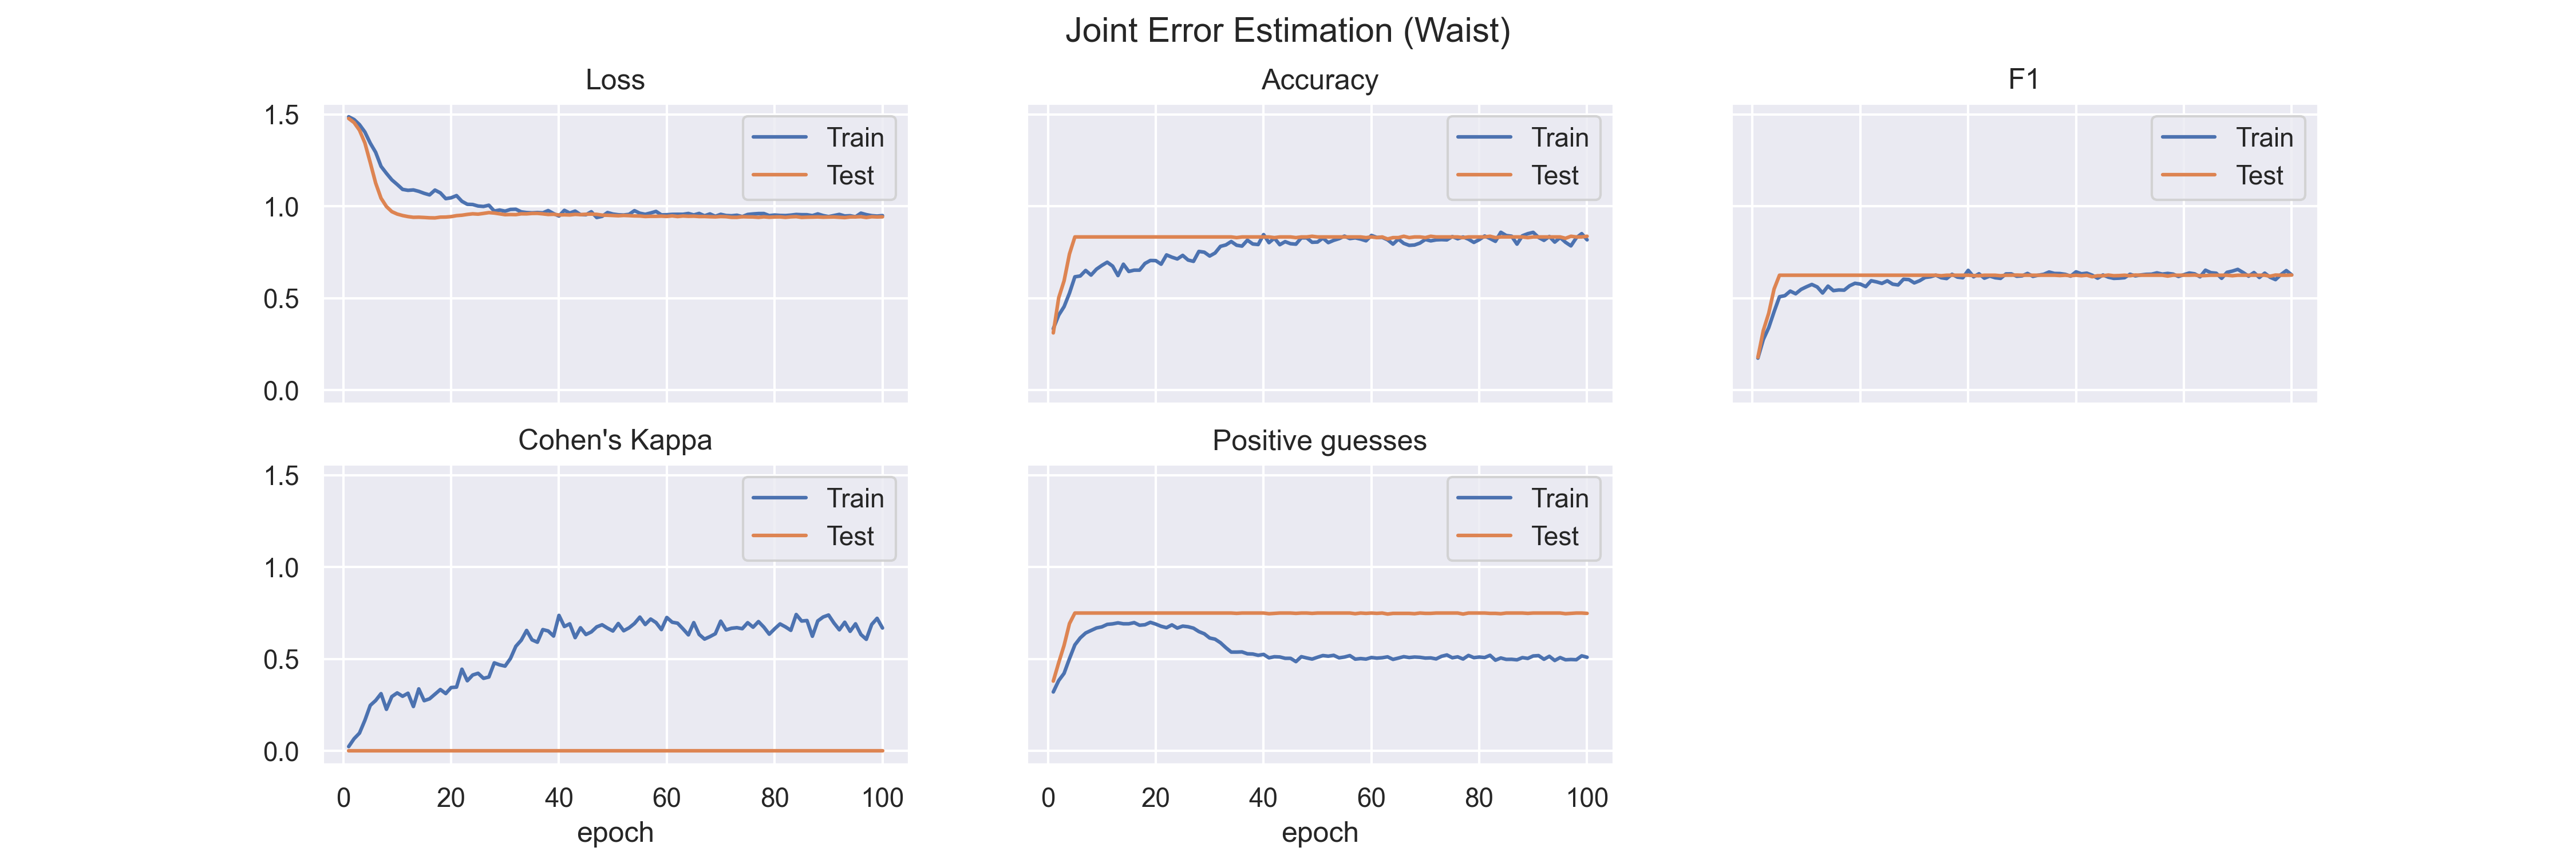
\includegraphics[width=\textwidth]{figures/Results/jt/JointErrorEstimation_Waist.png}
    \caption{Waist Error Estimation}
    \label{fig:waist_jt_ee}
  \end{subfigure}
  \hfill
  \begin{subfigure}[b]{0.47\linewidth}
      \centering
      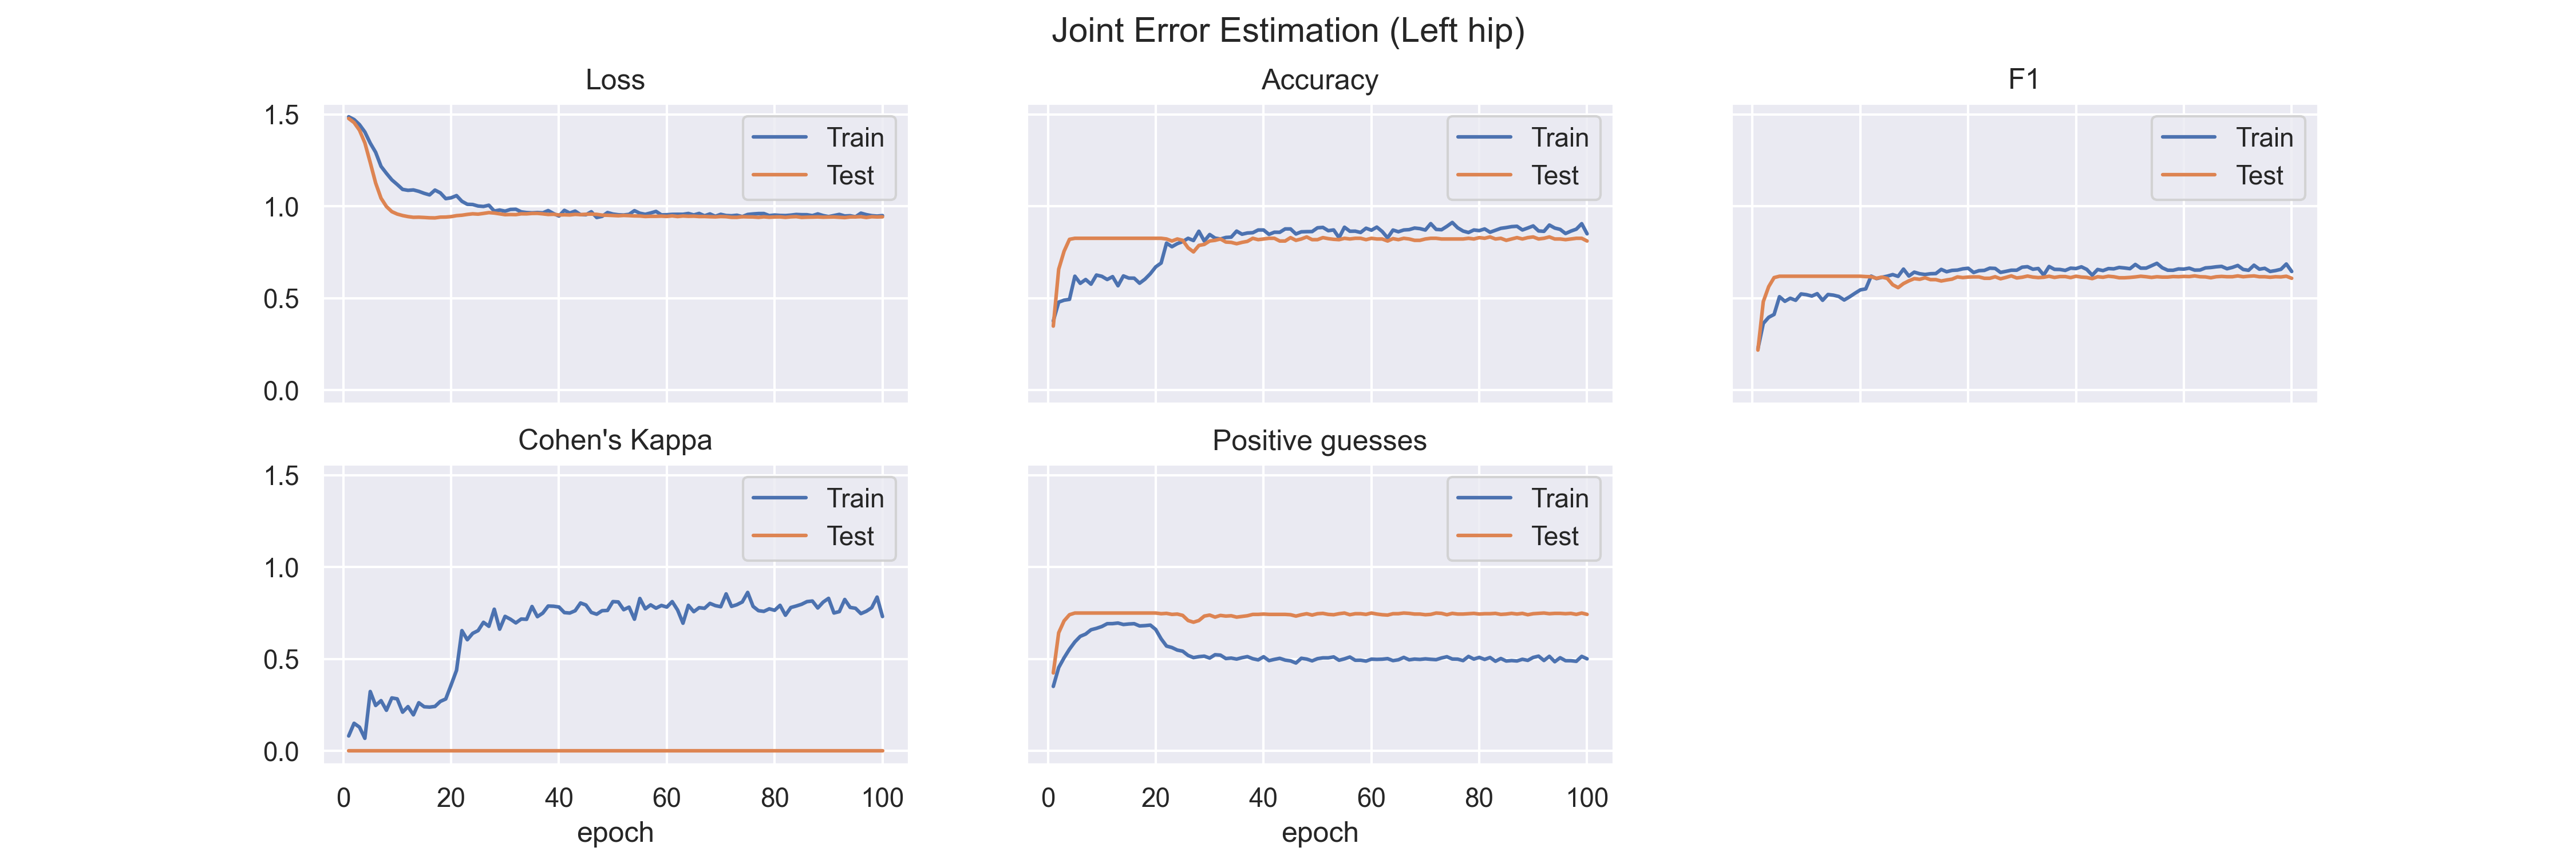
\includegraphics[width=\textwidth]{figures/Results/jt/JointErrorEstimation_Left hip.png}
      \caption{Left Hip Error Estimation}
      \label{fig:lehi_jt_ee}
  \end{subfigure}
  \hfill
  \begin{subfigure}[b]{0.47\linewidth}
      \centering
      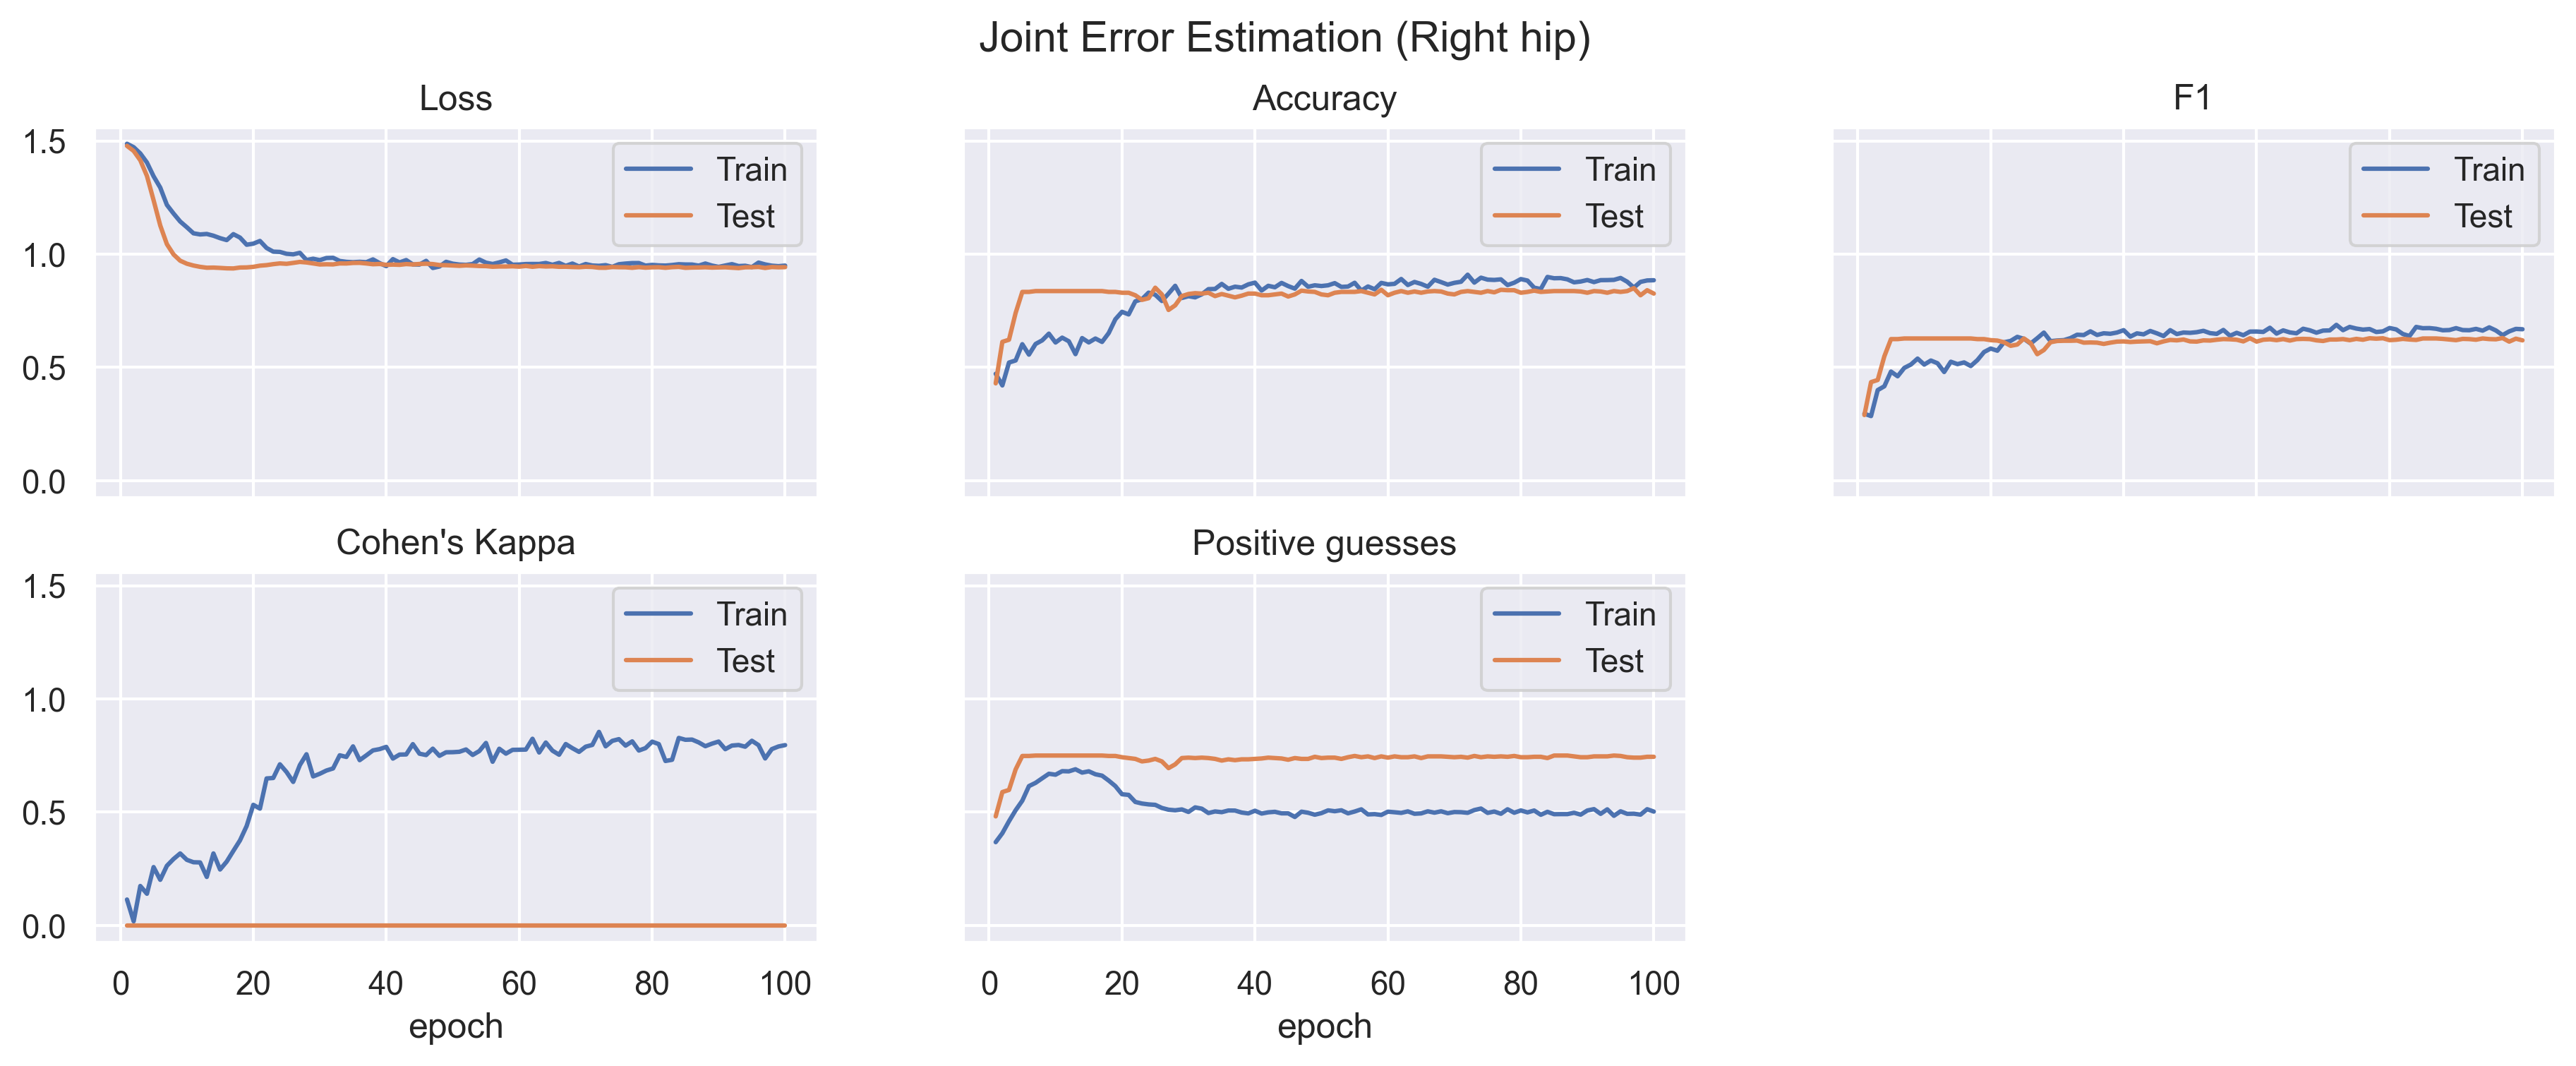
\includegraphics[width=\textwidth]{figures/Results/jt/JointErrorEstimation_Right hip.png}
      \caption{Right hip Error Estimation}
      \label{fig:rihi_jt_ee}
  \end{subfigure}
  \caption[Joint model training results]{The training results of the Joint error estimation model. (cont. 3)}
\end{figure}


\begin{figure}
  \centering
  \begin{subfigure}[b]{0.47\linewidth}
      \centering
      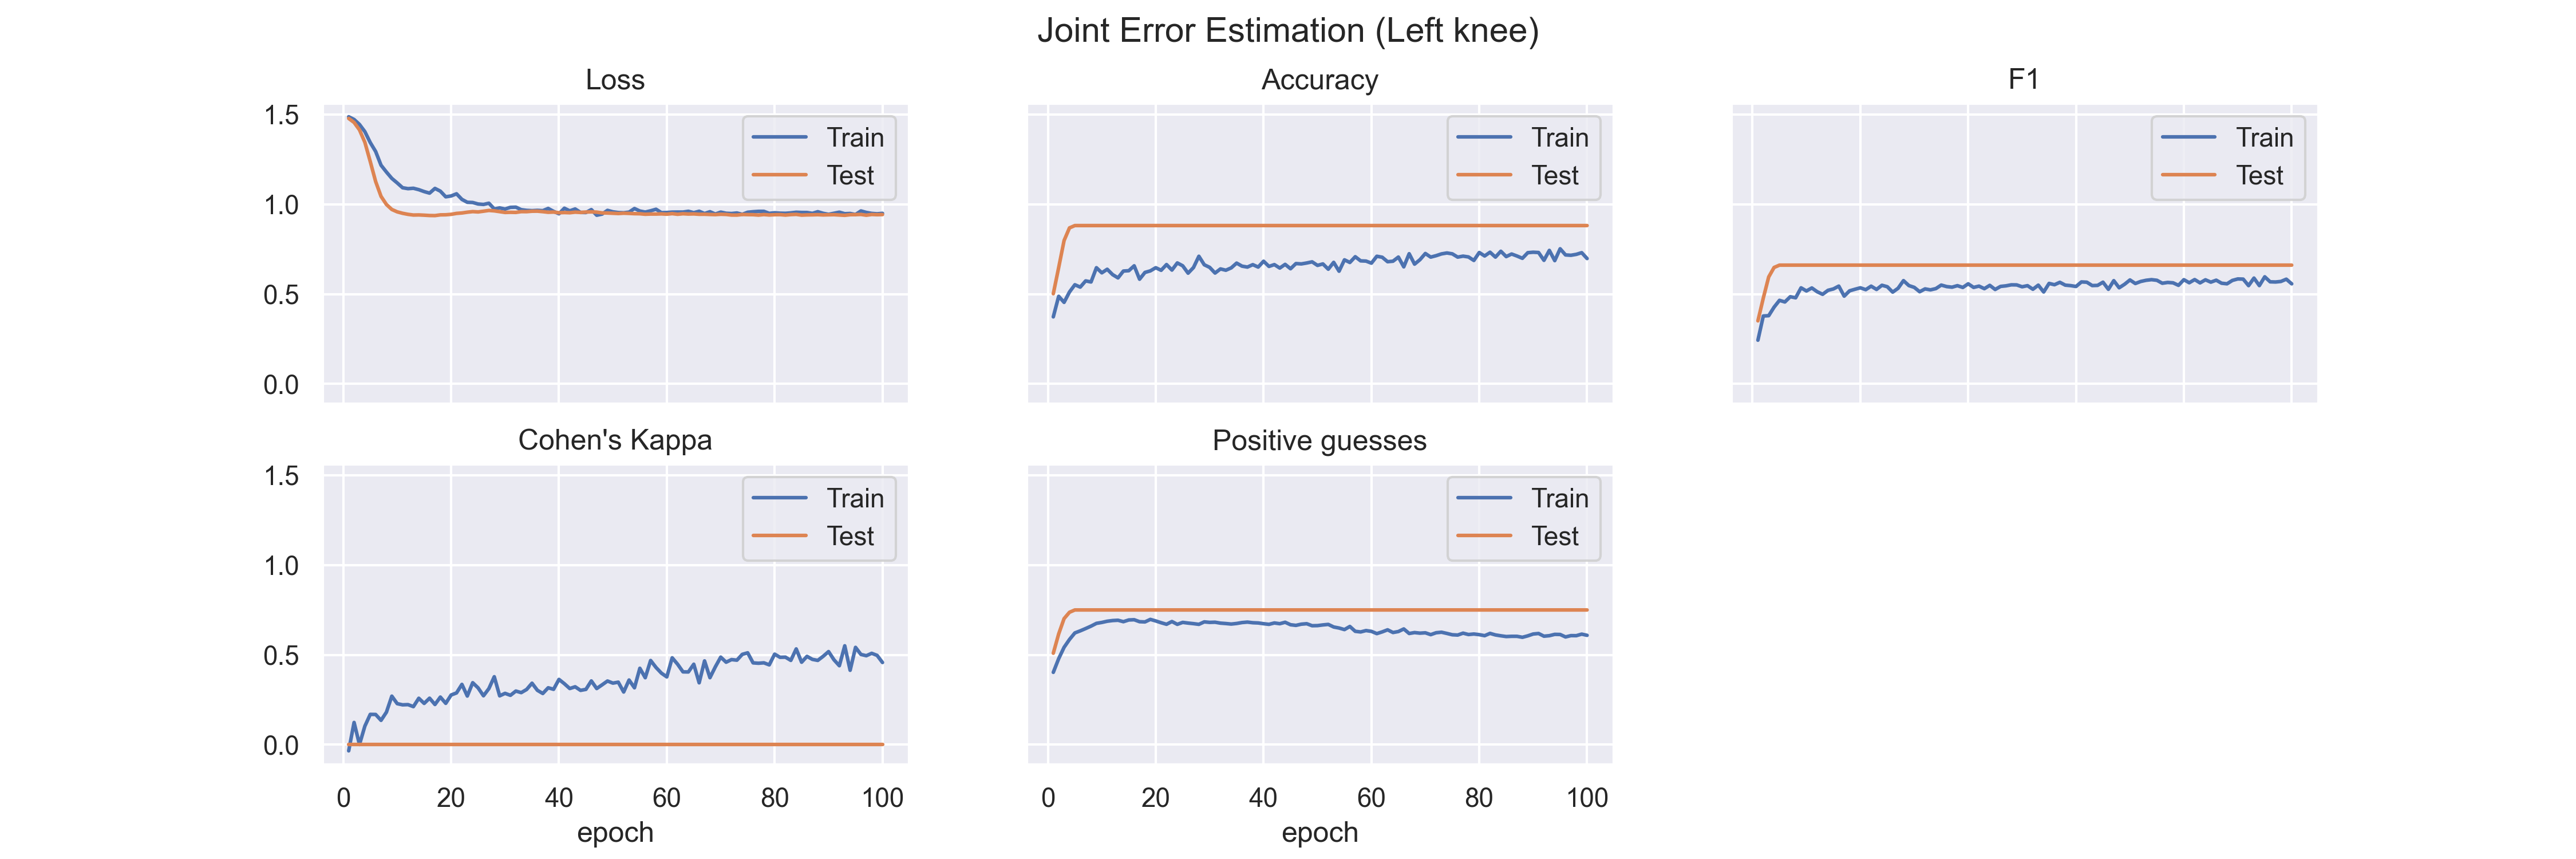
\includegraphics[width=\textwidth]{figures/Results/jt/JointErrorEstimation_Left knee.png}
      \caption{left Knee Error Estimation}
      \label{fig:lekn_jt_ee}
  \end{subfigure}
  \hfill
  \begin{subfigure}[b]{0.47\linewidth}
      \centering
      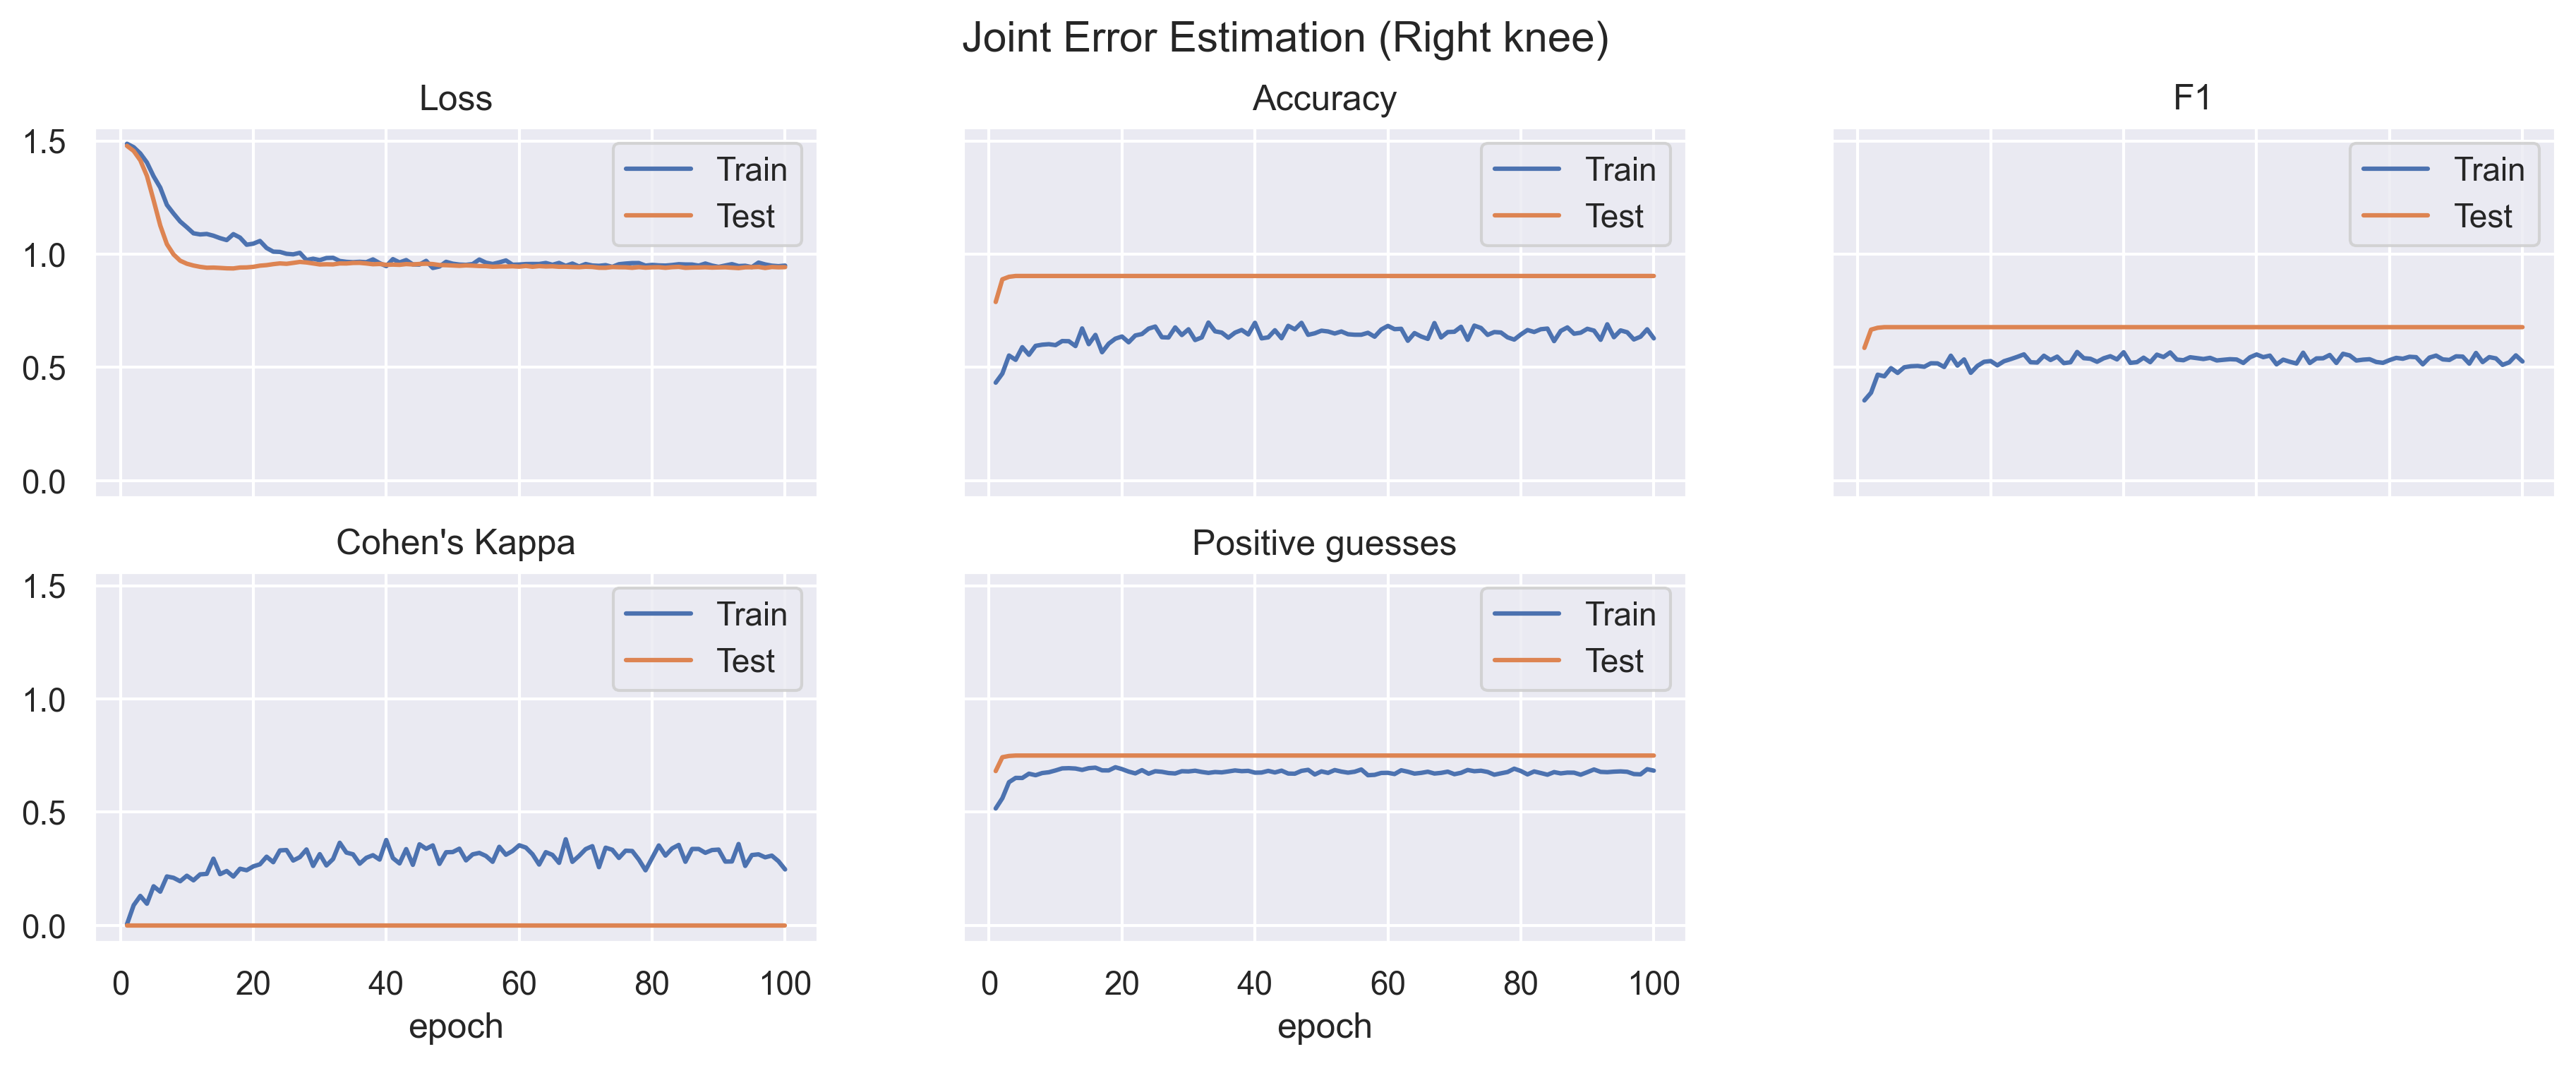
\includegraphics[width=\textwidth]{figures/Results/jt/JointErrorEstimation_Right knee.png}
      \caption{Right Knee Error Estimation}
      \label{fig:rikn_jt_ee}
  \end{subfigure}
  \hfill
  \begin{subfigure}[b]{0.47\linewidth}
      \centering
      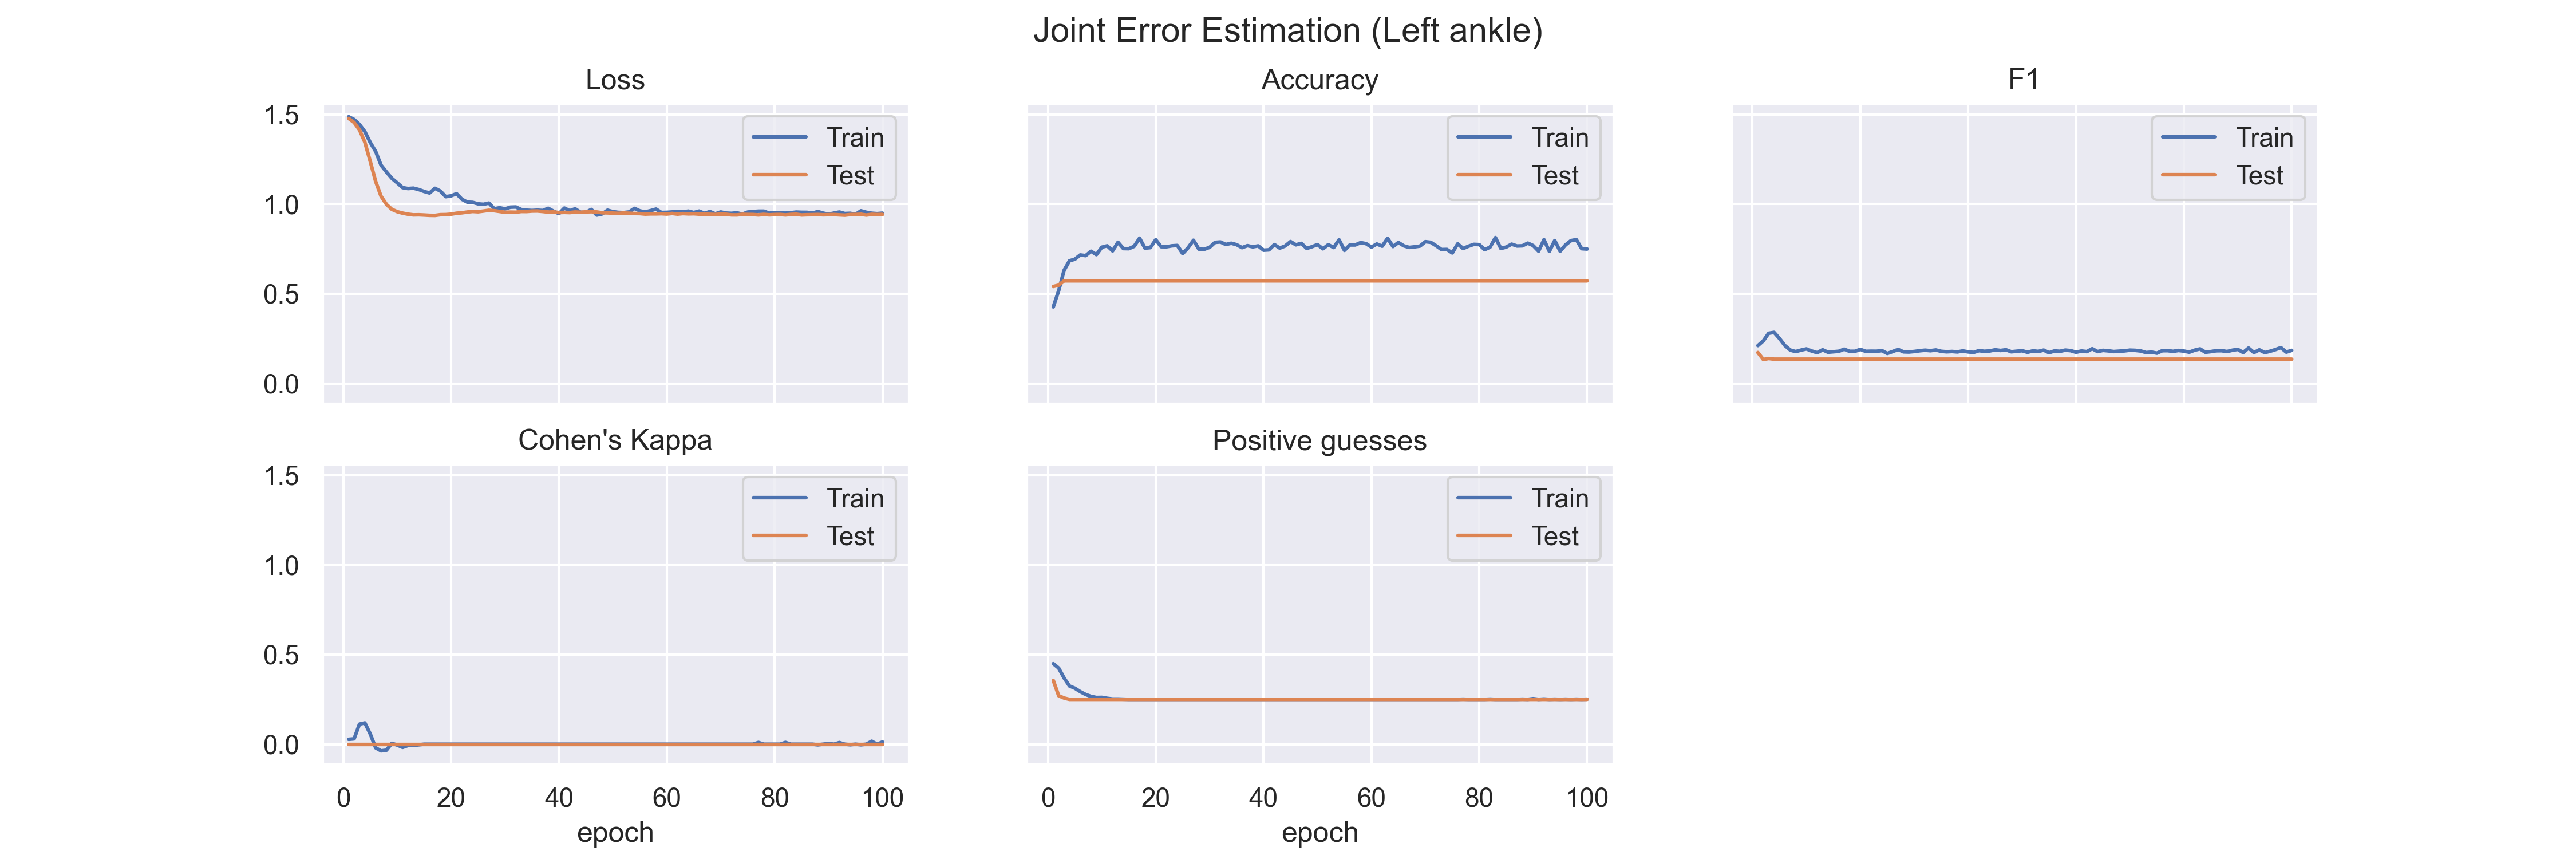
\includegraphics[width=\textwidth]{figures/Results/jt/JointErrorEstimation_Left ankle.png}
      \caption{Left Ankle Error Estimation}
      \label{fig:lean_jt_ee}
  \end{subfigure}
  \hfill
  \begin{subfigure}[b]{0.47\linewidth}
      \centering
      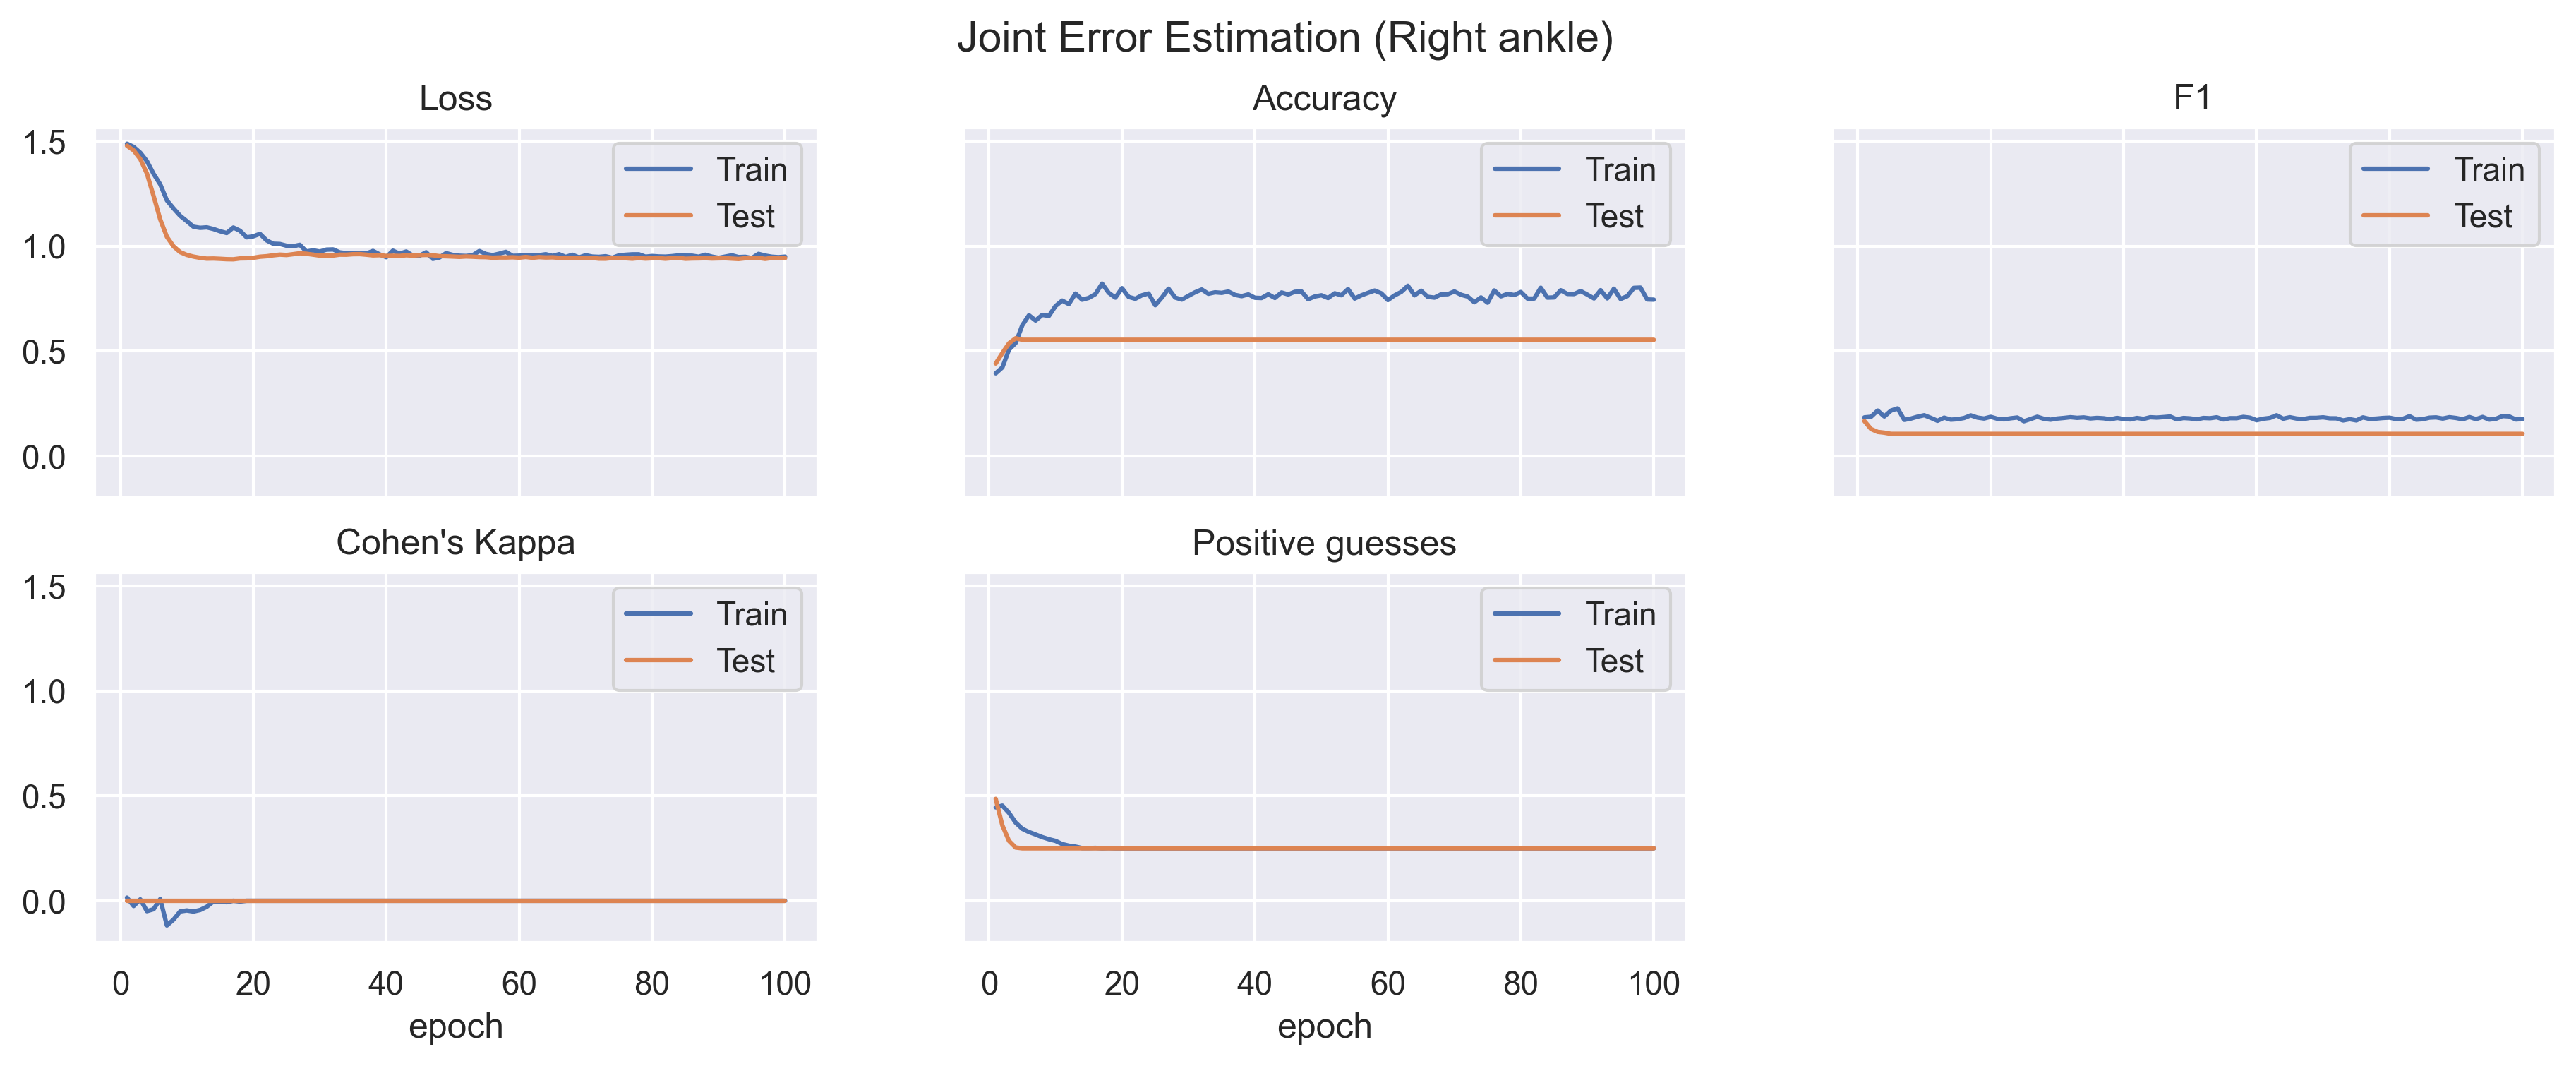
\includegraphics[width=\textwidth]{figures/Results/jt/JointErrorEstimation_Right ankle.png}
      \caption{Right Ankle Error Estimation}
      \label{fig:rian_jt_ee}
  \end{subfigure}
  \caption[Joint model training results]{The training results of the Joint error estimation model. (cont. 4)}
\end{figure}

\subsection{Confusion Matrix}

The confusion matrix of the joint model is shown in Figure \ref{fig:joint_confusion_matrix}(TODO: split that graph, its huge). It can be seen that the model only predicts the error label $0$ - No Error for most joints. This is because the model is overfitting.

\begin{figure}
  \centering
  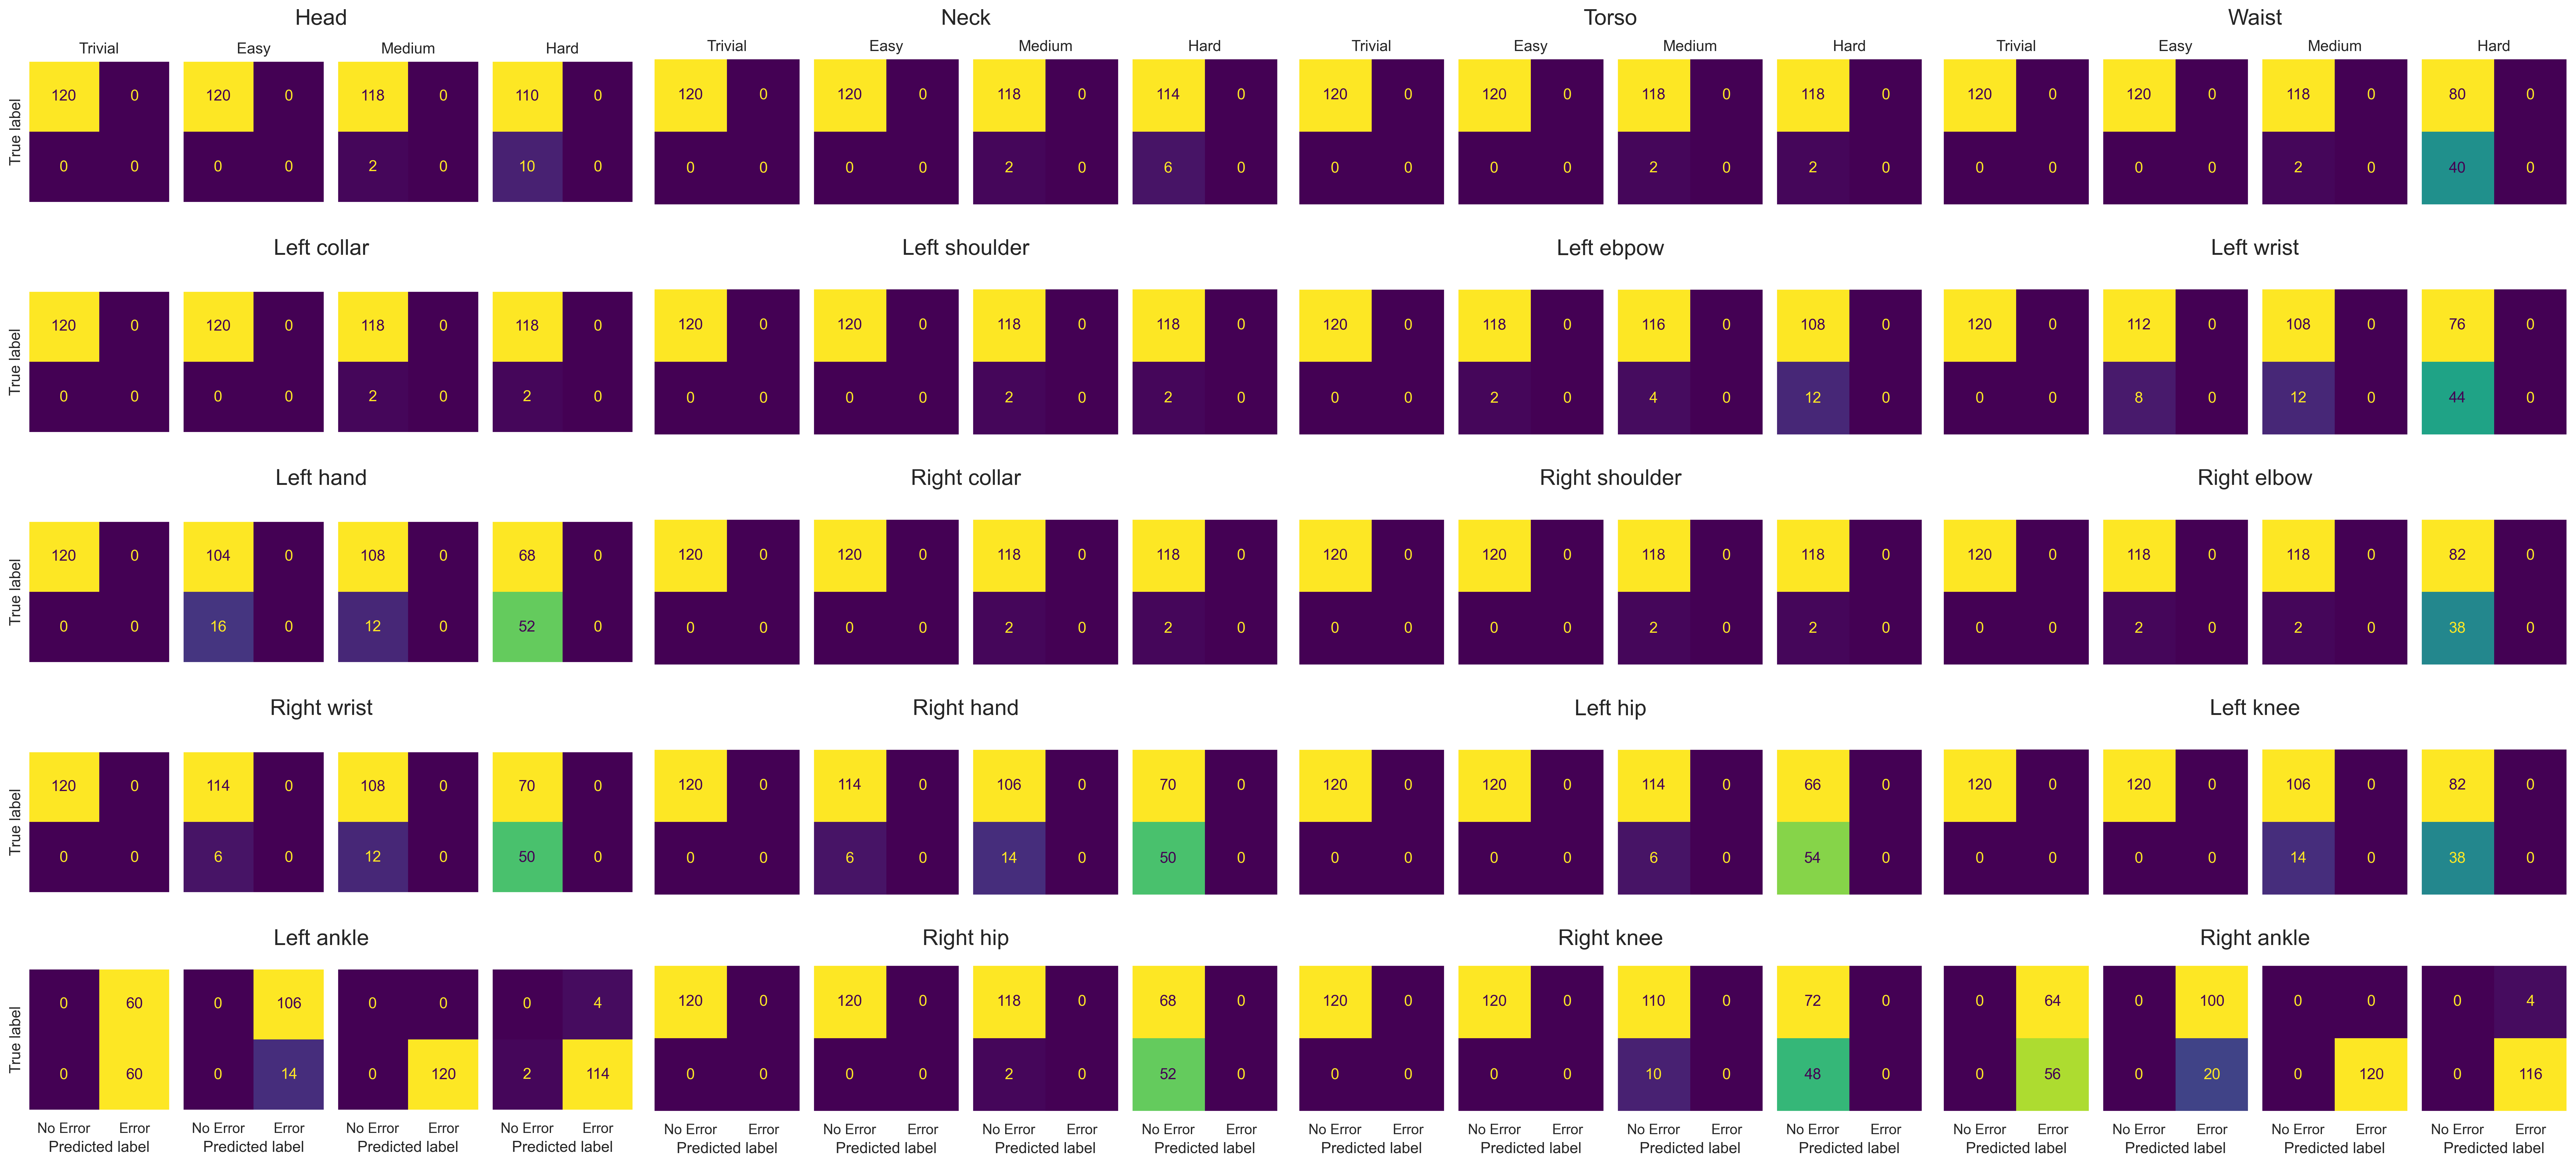
\includegraphics[width=0.5\textwidth]{figures/results/confusion/joints.png}
  \caption[Joint model confusion matrix]{The confusion matrix of the joint model.}
  \label{fig:joint_confusion_matrix}
\end{figure}

\subsection{Emulated Full Body}

As with the half-body Error estimator, the full body is emulated with the result of the limb error estimation. The results can be seen in Figure \ref{fig:joints_emulated_full_body}. 

\begin{figure}
    \centering
    %\includegraphics[width=0.8\textwidth]{figures/results/Half_Body/Emulated_Full_Body.png}
    \caption[Joint model with emulated Full Body results]{The results of the Joint model when emulating the full body results.}
    \label{fig:joints_emulated_full_body}
\end{figure}
  
\subsection{Emulated Half Body}

Additionally, the half body is emulated with the result of the limb error estimation. The Head, Torso, and Left and Right arms are considered the upper body, and the Left and Right legs are considered the lower body. The results of the model are shown in Figure \ref{fig:joints_emulated_half_body}.

\begin{figure}
    \centering
    %\includegraphics[width=0.8\textwidth]{figures/results/Half_Body/Emulated_Full_Body.png}
    \caption[Joint model with emulated Half Body results]{The results of the Joint model when emulating the half body results.}
    \label{fig:joints_emulated_full_body}
\end{figure}

\subsection{Emulated Limbs}

Finally, the results of the joint model are used to emulate the limb model. The results can be seen in Figure \ref{fig:joints_emulated_half_body}.

\begin{figure}
    \centering
    %\includegraphics[width=0.8\textwidth]{figures/results/Half_Body/Emulated_Full_Body.png}
    \caption[joint model with emulated Limb results]{The results of the Limb model when emulating the limb results.}
    \label{fig:joints_emulated_half_body}
\end{figure}